\Chapter{Qualitative Theory of Planar ODEs}
\label{Chap:PlanarQ}

\normalsize

Chapter~\ref{Chap:Planar} discussed three methods that are used to solve
planar systems of linear, constant coefficient, ordinary differential
equations.  The last method is based on similarity and the explicit
computation of the matrix exponential for certain normal form matrices.
This method depends crucially on the classification of $2\times 2$ matrices
up to similarity given in Chapter~\ref{Chap:Planar}, 
Theorem~\ref{T:putinform}.

In this chapter we explore qualitative features of phase portraits for planar 
linear systems of differential equations using similarity.  We find that the 
qualitative theory is completely determined by the eigenvalues and 
eigenvectors of the coefficient matrix --- which is not surprising given
that we can classify matrices up to similarity by just knowing their
eigenvalues and eigenvectors.  The set of planar phase portraits divides 
systems of linear differential equations into two camps: {\em hyperbolic\/} 
and {\em nonhyperbolic\/}.  The hyperbolic systems consist of {\em saddles\/},
{\em sinks\/} and {\em sources\/}, while the nonzero nonhyperbolic systems 
consist of {\em centers\/}, {\em saddle nodes\/}, and {\em shears\/}.


\Section{Sinks, Saddles, and Sources} \label{S:6.7}

The qualitative theory of autonomous differential equations begins with
the observation that many important properties of solutions to constant
coefficient systems of differential equations
\begin{equation} \label{e:C2}
\frac{dX}{dt}=CX
\end{equation}
are unchanged by similarity.

Begin by noting that the origin is always an equilibrium for \Ref{e:C2}
and suppose that $C$ is a $2\times 2$ matrix.  The origin for \Ref{e:C2}
is called a {\em sink\/}\index{sink} if the eigenvalues of $C$ both have
negative real
part and a {\em source\/}\index{source} if the eigenvalues both have
positive real part.
When $C$ has one eigenvalue of each sign, the origin is called a
{\em saddle}\index{saddle}.

Now suppose that $B$ is a $2\times 2$ matrix that is similar to $C$.
Lemma~\ref{L:simdettr} of Chapter~\ref{Chap:Planar} states that $B$ and
$C$ have the same eigenvalues.  It follows that if the origin is a saddle
for \Ref{e:C2}, then it is a saddle for $\dot{X}=BX$.  Similar statements
hold for sinks and sources.

\subsection*{Asymptotic Stability}

We now discuss asymptotic stability of the origin in linear systems.
Recall from our discussion in Section~\ref{sec:UncoupledLS} 
that the origin is {\em asymptotically stable\/} \index{stability!asymptotic}
if every trajectory $X(t)$ beginning at an initial condition near the
origin stays near $0$ for all positive $t$, and
\[
\lim_{t\to\infty}X(t) = 0.
\]
Recall also from Lemma~\ref{L:simsoln} of Chapter~\ref{Chap:Planar} that
if $B=P\inv CP$, then $P\inv X(t)$ is a solution to $\dot{X}=BX$ whenever
$X(t)$ is a solution to \Ref{e:C2}.  Since $P\inv$ is a matrix of constants
that do not depend on $t$, it follows that
\[
\lim_{t\to\infty}X(t) = 0 \Longleftrightarrow \lim_{t\to\infty}P\inv X(t) = 0.
\]
So the origin is asymptotically stable for $\dot{X}=BX$ if and only if it is
asymptotically stable for \Ref{e:C2}.  With this observation in hand, we
prove that sinks are stable.

\begin{thm}  \label{C:asympstlin}
If the eigenvalues of $C$ have negative real part, then the origin
is an asymptotically stable equilibrium\index{equilibrium} for \Ref{e:C2}.
If one of the
eigenvalues of $C$ has positive real part, then the origin is unstable.
\end{thm}

\proof  This proof is based on the closed form of solutions given in
Section~\ref{S:6.5}.   The remark preceding this theorem states that we
need only prove this theorem for differential equations up to similarity.

\noindent (a) \quad If the eigenvalues $\lambda_1$ and $\lambda_2$ are real
and there are two independent eigenvectors, then Chapter~\ref{Chap:Planar},
Theorem~\ref{T:putinform} states that the matrix $C$ is similar to the
diagonal matrix
\[
B = \mattwoc{\lambda_1}{0}{0}{\lambda_2}.
\]
The general solution to the differential equation $\dot{X}=BX$ is
\[
x_1(t) = \alpha_1e^{\lambda_1 t} \AND x_2(t) = \alpha_2e^{\lambda_2 t}.
\]
Since
\[
\lim_{t\to\infty}e^{\lambda_1 t} = 0  = \lim_{t\to\infty}e^{\lambda_2 t},
\]
when $\lambda_1$ and $\lambda_2$ are negative, it follows that
\[
\lim_{t\to\infty} X(t) = 0
\]
for all solutions $X(t)$, and the origin is asymptotically stable.  Note that
if one of the eigenvalues, say $\lambda_1$, is positive then $x_1(t)$ will
undergo exponential growth and the origin is unstable.

\noindent (b) \quad If the eigenvalues of $C$ are the complex conjugates
$\sigma\pm i\tau$ where $\tau\neq 0$, then Chapter~\ref{Chap:Planar},
Theorem~\ref{T:putinform} states that after a similarity transformation
\Ref{e:C2} has the form
\[
\dot{X} = \mattwo{\sigma}{-\tau}{\tau}{\sigma}X,
\]
and solutions for this equation have the form \Ref{e:exp0ev} of
Chapter~\ref{Chap:Planar}, that is,
\[
X(t) = e^{\sigma t}
\mattwo{\cos(\tau t)}{-\sin(\tau t)}{\sin(\tau t)}{\cos(\tau t)}X_0
= e^{\sigma t}R_{\tau t}X_0,
\]
where $R_{\tau t}$ is a rotation matrix\index{rotation!matrix}
(recall \Ref{e:rotmat} of
Chapter~\ref{chap:matrices}).  It follows that as time evolves
the vector $X_0$ is rotated about the origin and then expanded or contracted
by the factor $e^{\sigma t}$.  So when $\sigma<0$, $\lim_{t\to\infty} X(t)=0$
for all solutions $X(t)$.  Hence the origin is asymptotically stable.  Note
that when $\sigma>0$ solutions spiral away from the origin.

\noindent (c) \quad If the eigenvalues are both equal to $\lambda_1$
and if there is only one independent eigenvector, then
Chapter~\ref{Chap:Planar}, Theorem~\ref{T:putinform} states that after a
similarity transformation \Ref{e:C2} has the form
\[
\dot{X} = \mattwo{\lambda_1}{1}{0}{\lambda_1}X,
\]
whose solutions are
\[
X(t) = e^{t\lambda}\mattwoc{1}{t}{0}{1} X_0
\]
using \Ref{e:expshear} of Chapter~\ref{Chap:Planar}. Note that the functions
$e^{\lambda_1 t} \AND te^{\lambda_1 t}$ both have limits equal to zero as
$t\to\infty$.  In the second case, use l'H\^{o}spital's rule and the
assumption that $-\lambda_1>0$ to compute
\[
\lim_{t\to\infty} \frac{t}{e^{-\lambda_1 t}} =
  -\lim_{t\to\infty} \frac{1}{\lambda_1 e^{-\lambda_1 t}} = 0.
\]
Hence $\lim_{t\to\infty} X(t) =0$ for all solutions $X(t)$ and the origin
is asymptotically stable.  Note that initially $||X(t)||$ can grow since
$t$ is increasing.  But eventually exponential decay wins out and solutions
limit on the origin.   Note that solutions grow exponentially when
$\lambda_1>0$.  \qed

It is instructive to note how the time series $x_1(t)$ damps down to the
origin in the three cases listed in Theorem~\ref{C:asympstlin}.
In Figure~\ref{F:oscil} we present the time series for the three
coefficient matrices:
\[
C_1 = \mattwo{-2}{0}{0}{-1} \qquad
C_2 = \mattwo{-1}{-55}{55}{-1} \qquad
C_3 = \mattwo{-2}{1}{0}{-2}.
\]
In this figure, we can see the exponential decay to zero associated with the
unequal real eigenvalues of $C_1$; the damped oscillation associated with the
complex eigenvalues of $C_2$; and the initial growth of the time series due
to the $te^{-2t}$ term followed by exponential decay to zero in the equal
eigenvalue $C_3$ example.

\begin{figure}[htb]
           \centerline{%
           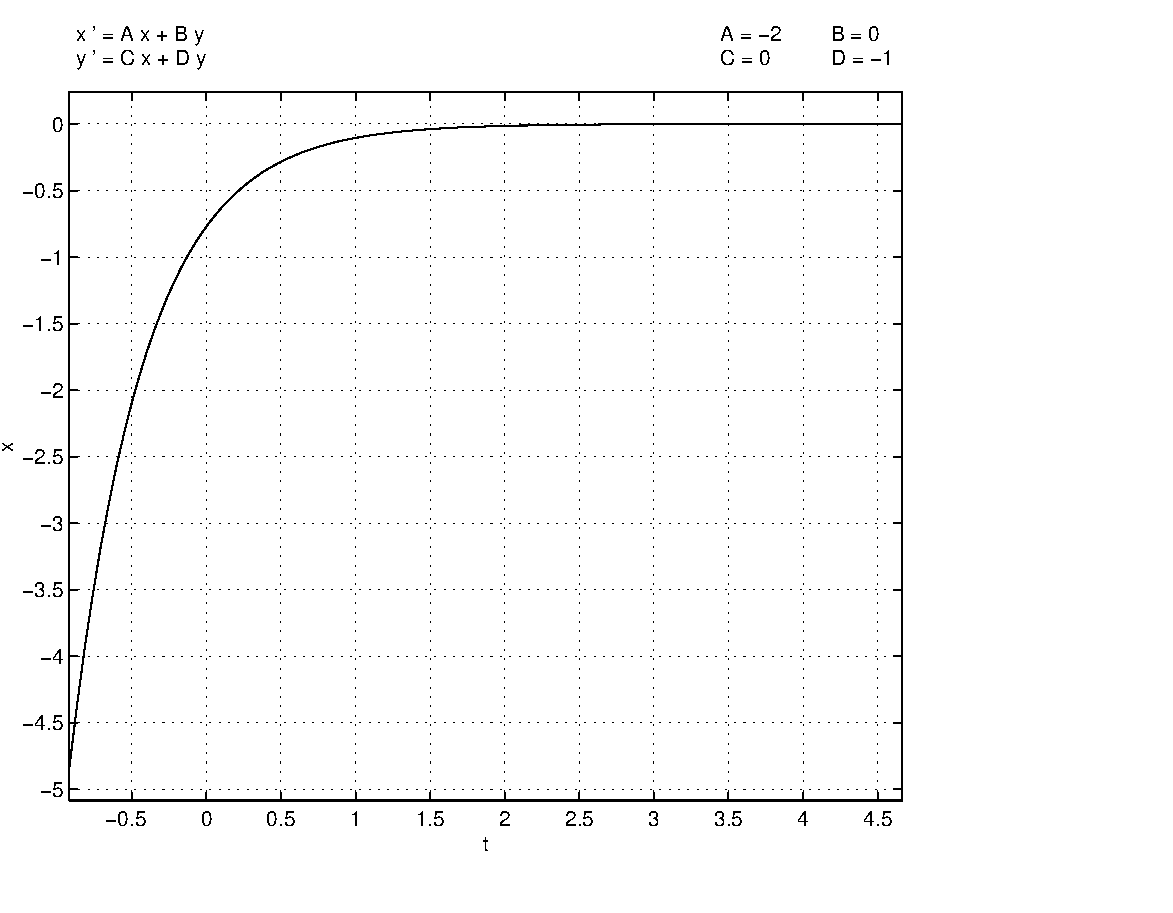
\psfig{file=figures/expdamp.eps,width=2.2in}
	   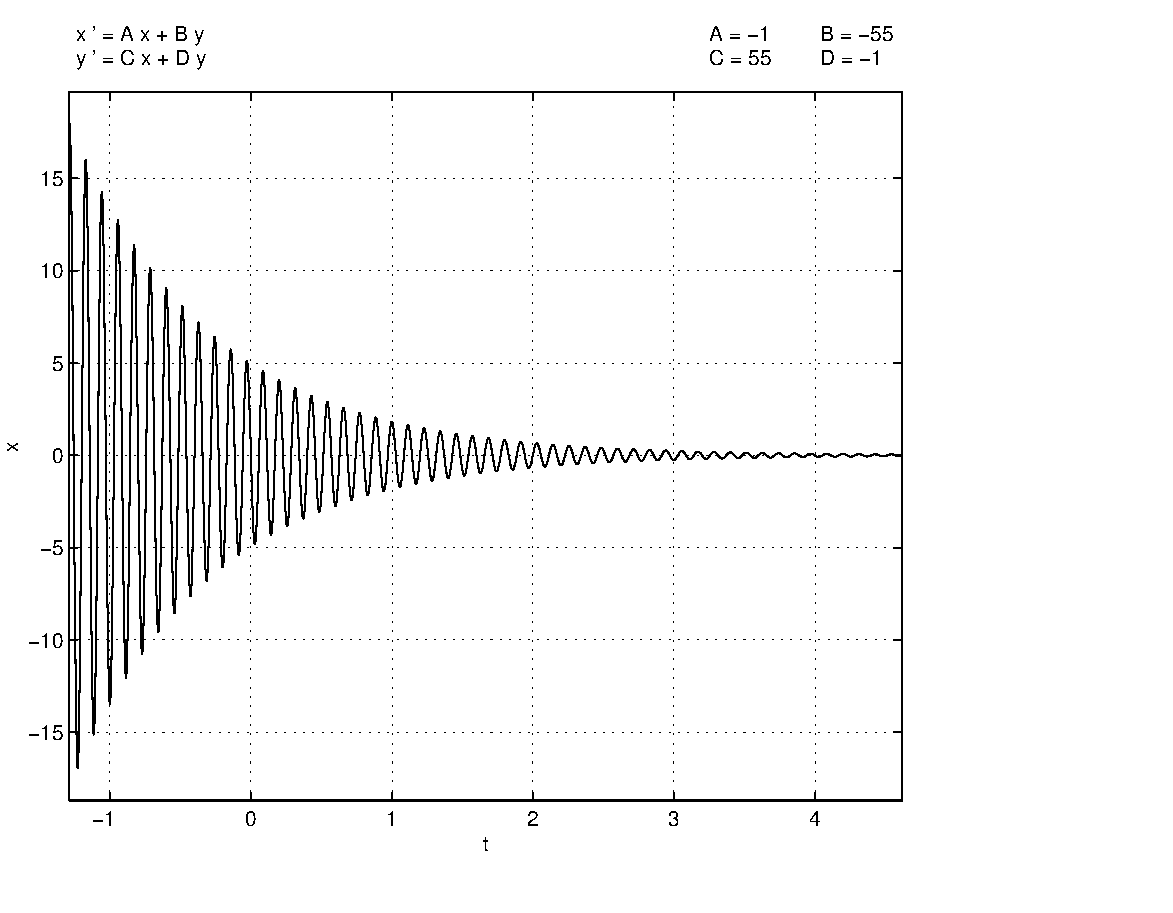
\psfig{file=figures/oscil.eps,width=2.2in}
	   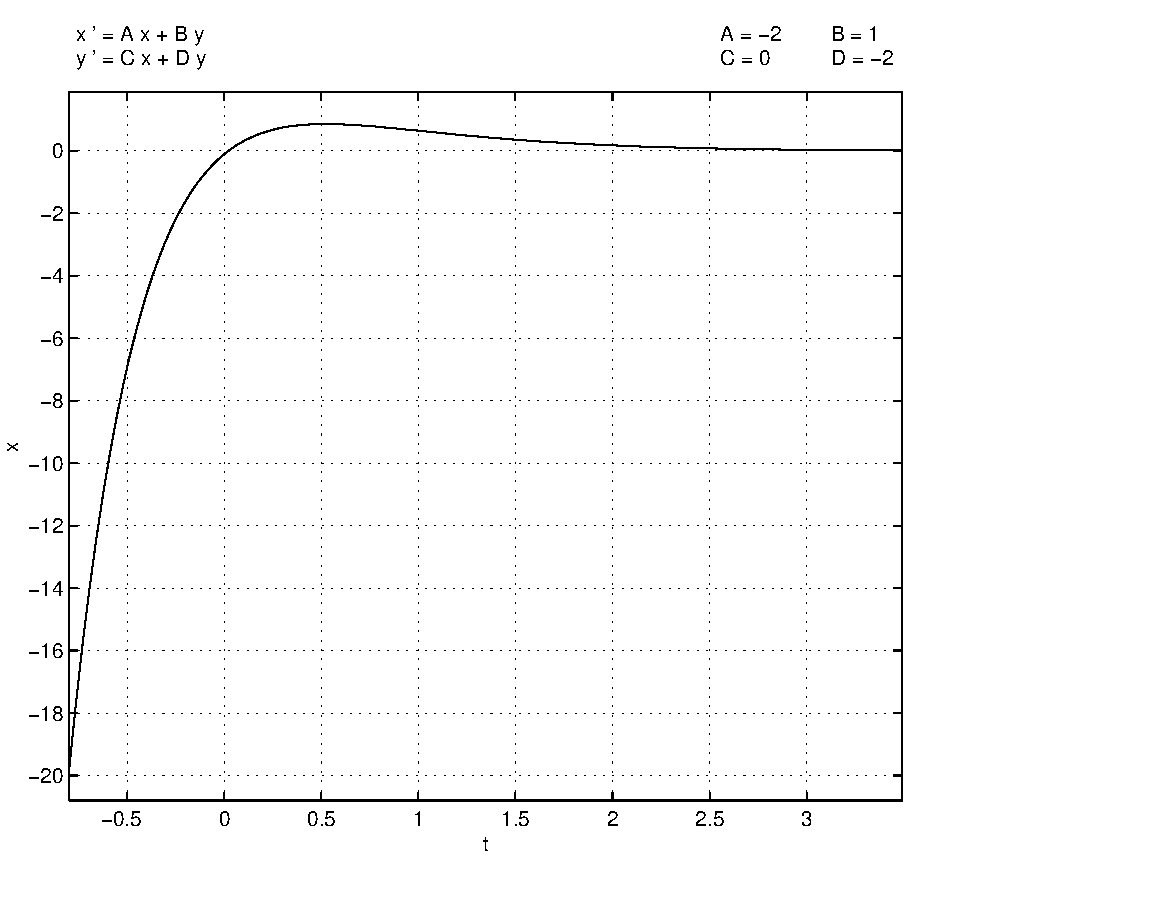
\psfig{file=figures/grdecay.eps,width=2.2in}}
           \caption{Time series for different sinks.}
           \label{F:oscil}
\end{figure}


\subsubsection*{Linear Stability}

Saddles, sinks, and sources are distinguished by the stability of the
origin.  In Theorem~\ref{C:asympstlin} we showed that the origin is
asymptotically stable if the eigenvalues have negative real part, that is,
if the origin is a sink.  There is another term that is commonly used and
is synonymous with sink.
\begin{Def} \label{D:linstablin}
The origin is a {\em linearly stable\/} equilibrium of \Ref{e:C2} if the
eigenvalues of $C$ have negative real part.
\end{Def}\index{stability!linear}
So Theorem~\ref{C:asympstlin} may be restated as: linear stability
implies asymptotic stability of the origin.

\subsubsection*{Sources Versus Sinks}

The explicit form of solutions to planar linear systems shows that solutions
with initial conditions near the origin grow exponentially in forward time
when the origin of \Ref{e:C2} is a source.  We can prove this point
geometrically, as follows.

The phase planes of sources and sinks are almost the same; they have the
same trajectories but the arrows are reversed.  To verify this point, note
that
\begin{equation}  \label{e:C3}
\dot{X}=-CX
\end{equation}
is a sink when \Ref{e:C2} is a source; observe that the trajectories of
solutions of \Ref{e:C2} are the same as those of \Ref{e:C3} --- just with
time running backwards.  For let $X(t)$ be a solution to \Ref{e:C2}; then
$X(-t)$ is a solution to \Ref{e:C3}.   See Figure~\ref{F:SS} for plots of
$\dot{X}=BX$ and $\dot{X}=-BX$ where
\begin{equation}  \label{E:SS}
B = \mattwo{-1}{-5}{5}{-1}.
\end{equation}

So when we draw schematic phase portraits\index{phase!portrait}
for sinks\index{phase!portrait!for a sink}, we automatically know
how to draw schematic phase portraits for
sources\index{phase!portrait!for a source}.  The trajectories are
the same --- but the arrows point in the opposite direction.

\begin{figure}[htb]
           \centerline{%
	   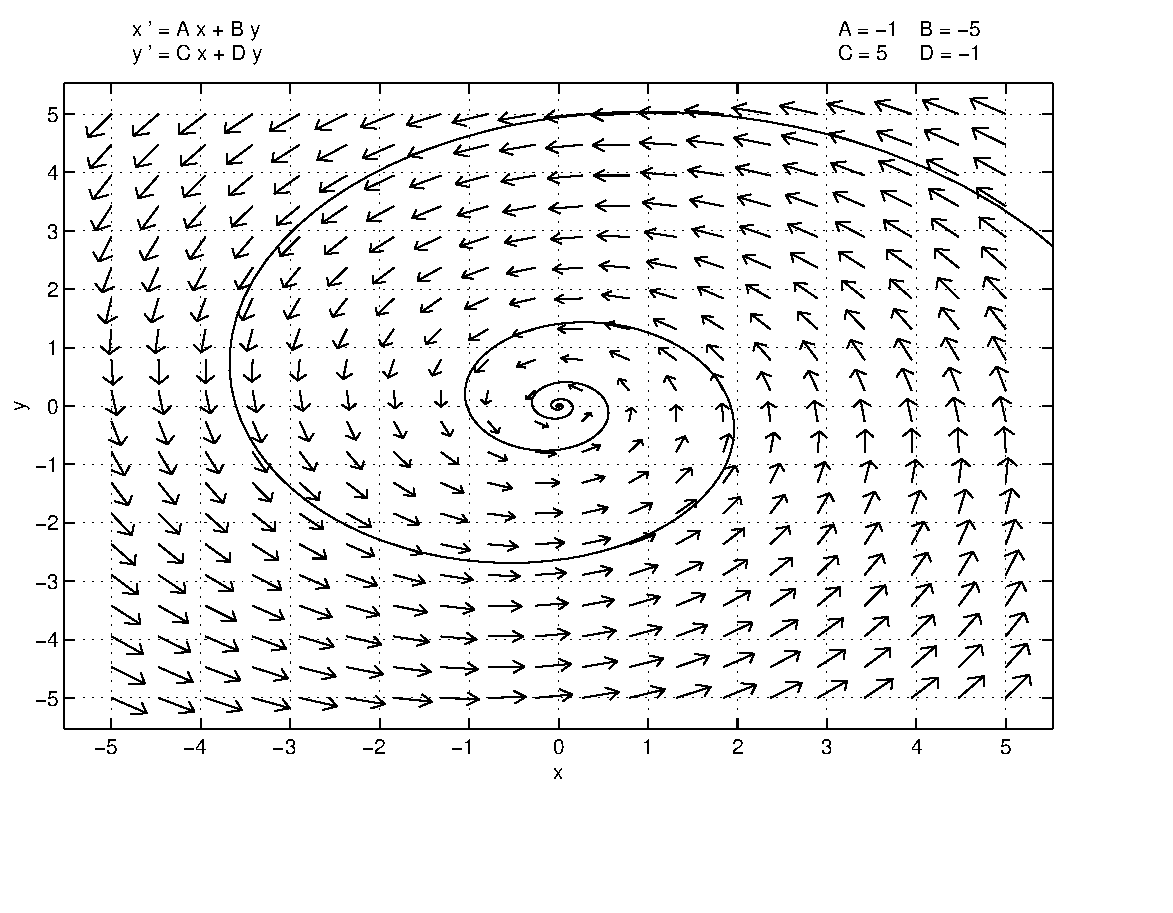
\psfig{file=figures/asink.eps,width=3.2in}
           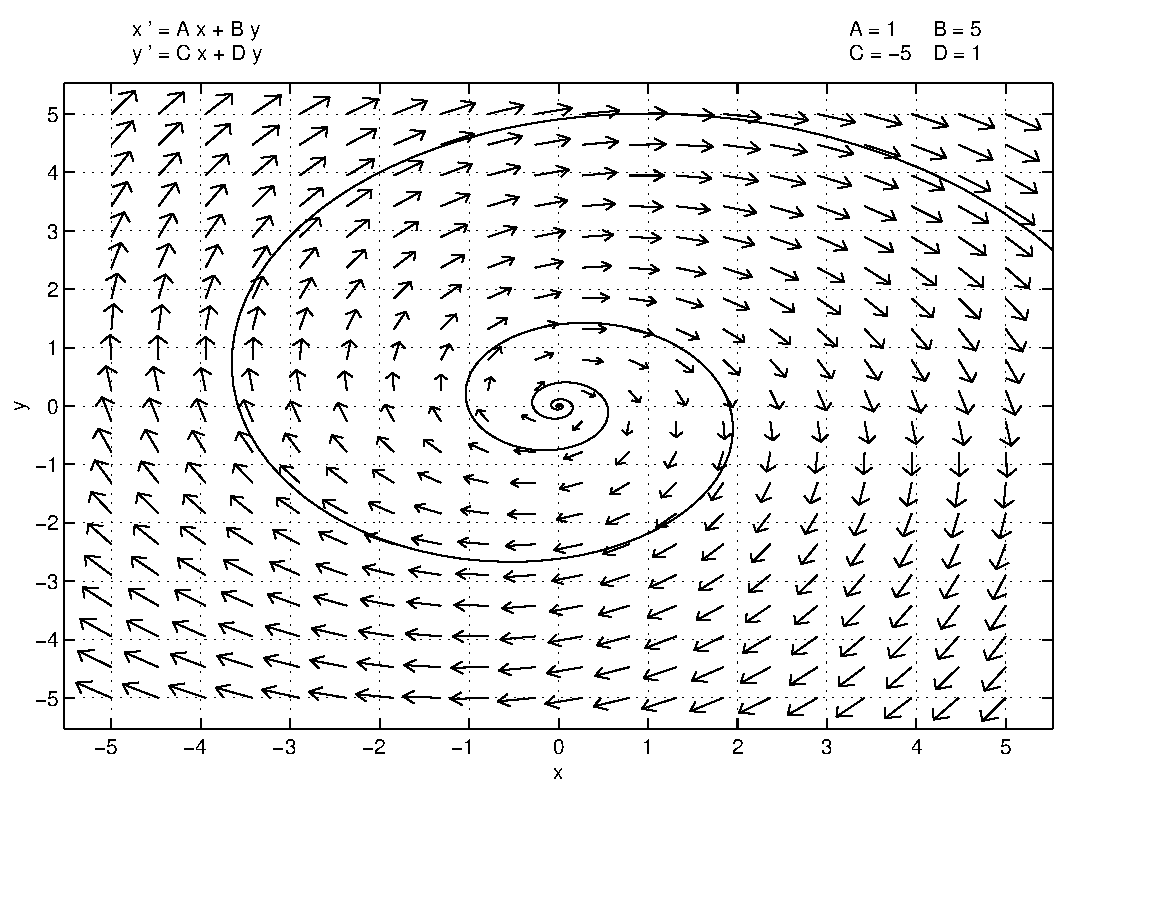
\psfig{file=figures/asource.eps,width=3.2in}}
           \caption{(Left) Sink $\dot{X}=BX$ where $B$ is given in
\protect{\Ref{E:SS}}.  (Right) Source $\dot{X}=-BX$.}
           \label{F:SS}
\end{figure}


\subsection*{Phase Portraits for Saddles}
\index{phase!portrait!for a saddle}

Next we discuss the phase portraits of linear saddles.  Using
{\sf pplane5}\index{\computer!pplane5}, draw the phase portrait
of the saddle
\begin{equation}  \label{e:saddlet}
\begin{array}{rcl}
\dot{x} & = & 2x+y\\
\dot{y} & = & -x-3y,
\end{array}
\end{equation}
as in Figure~\ref{F:linsaddle}.  The important feature of saddles
is that there are special trajectories (the eigendirections) that
limit on the origin in either forward or backward time.

\begin{figure}[htb]
           \centerline{%
	   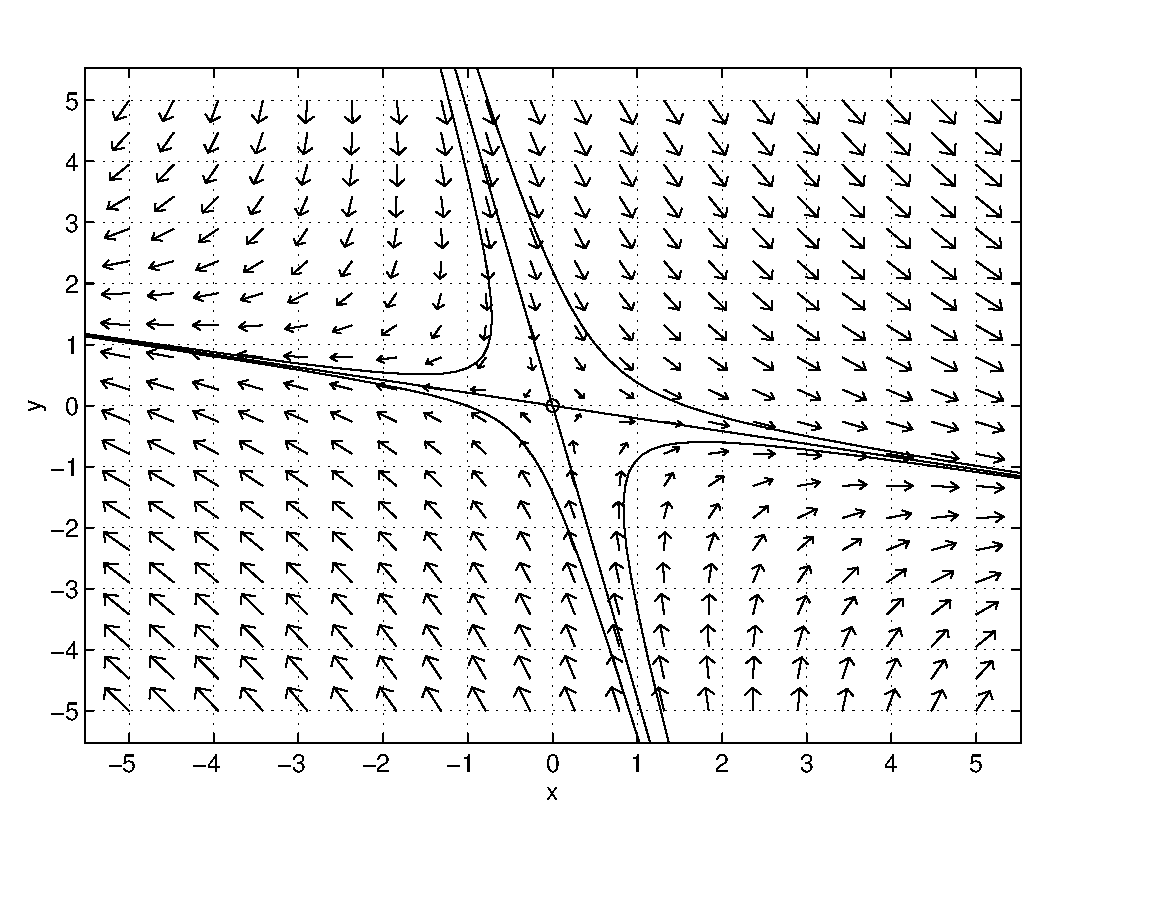
\psfig{file=figures/linpnb.eps,width=3.5in}
           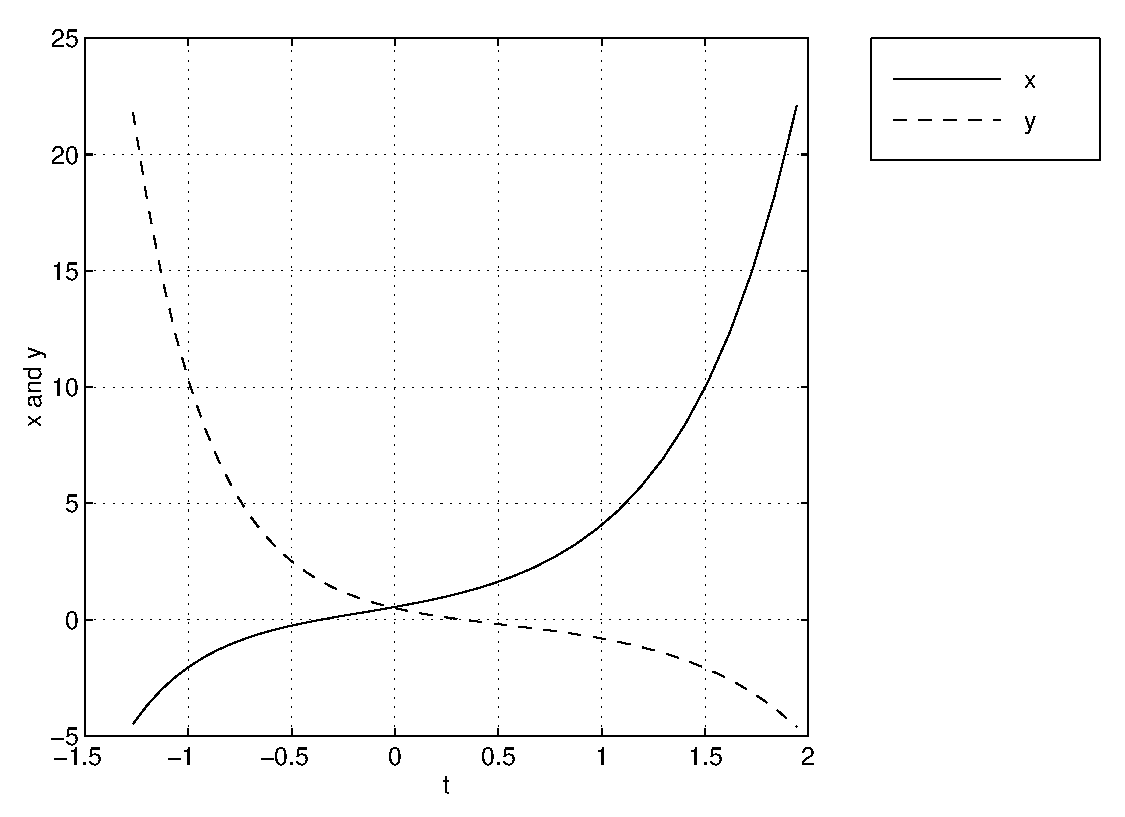
\psfig{file=figures/linpnts.eps,width=3.5in}}
           \caption{(Left) Saddle phase portrait.
	(Right) First quadrant solution time series.}
           \label{F:linsaddle}
\end{figure}

\begin{Def} \label{D:stablemfld}
The {\em stable manifold\/} or {\em stable orbit\/} of a saddle consists of
those trajectories that limit on the origin in forward time; the
{\em unstable manifold\/} or {\em unstable orbit\/} of a saddle consists of
those trajectories that limit on the origin in backward time.
\end{Def}
\index{stable!manifold} \index{unstable!manifold}
\index{stable!orbit} \index{unstable!orbit}

Let $\lambda_1<0$ and $\lambda_2>0$ be the eigenvalues of a saddle with
associated eigenvectors $v_1$ and $v_2$.  The stable orbits are given by the
solutions $X(t) = \pm e^{\lambda_1 t}v_1$ and the unstable orbits are given
by the solutions $X(t) = \pm e^{\lambda_2 t}v_2$.

\subsubsection*{Stable and Unstable Orbits using {\sf pplane5}}

The program {\sf pplane5} is programmed to draw the stable and unstable
orbits of a saddle on command. Although the principal use of this
feature is seen when analyzing nonlinear systems, it is useful to
introduce this feature here.  As an example, load the linear system
\Ref{e:saddlet} into {\sf pplane5} and click on {\sf Proceed}.  Now
pull down the {\sf PPLANE5 Options} menu and click on {\sf Find an
equilibrium}.  Click the cross hairs in the {\sf PPLANE5 Display}
window on a point near the origin; {\sf pplane5} responds by
opening a new window --- the {\sf PPLANE5 Equilibrium point data}
window --- and by putting a small yellow circle about the
origin.  The circle indicates that the numerical algorithm
programmed into {\sf pplane5} has detected an equilibrium near
the chosen point. A new window opens and displays the message
{\sf There is a saddle point at} $(0,0)$.  This window also displays the
coefficient matrix (called the Jacobian for reasons that will be discussed
in Section~\ref{S:linearization}) at the equilibrium and its eigenvalues
and eigenvectors.  This process numerically verifies that the origin
is a saddle (a fact that could have been verified in a more
straightforward way).

Now pull down the {\sf PPLANE5 Options} menu again and click on
{\sf Plot stable and unstable orbits}.  Next click on the mouse
when the cross hairs are within the yellow circle and {\sf
pplane5} responds by drawing the stable and unstable orbits.
The result is shown in Figure~\ref{F:linsaddle}(left).
On this figure we have also plotted one trajectory
from each quadrant; thus obtaining the phase portrait of a saddle.
On the right of Figure~\ref{F:linsaddle} we have plotted a
time series of the first quadrant solution.  Note how the $x$
time series increases exponentially to $+\infty$ in forward time and 
the $y$ time series decreases in forward time while going exponentially 
towards $-\infty$.  The two time series together
give the trajectory $(x(t),y(t))$ that in forward time is asymptotic
to the line given by the unstable eigendirection.



\EXER

\TEXER


\noindent In Exercises~\ref{E:stabmata} -- \ref{E:stabmatc} determine
whether or not the equilibrium at the origin in the system of differential
equations $\dot{X}=CX$ is asymptotically stable.
\begin{exercise} \label{E:stabmata}
$C=\mattwo{1}{2}{4}{1}$.
\end{exercise}
\begin{exercise} \label{E:stabmatb}
$C=\mattwo{-1}{2}{-4}{-1}$.
\end{exercise}
\begin{exercise} \label{E:stabmatc}
$C=\mattwo{2}{1}{1}{-5}$.
\end{exercise}

\noindent In Exercises~\ref{E:sisasoa} -- \ref{E:sisasof} determine
whether the equilibrium at the origin in the system of differential
equations $\dot{X}=CX$ is a sink, a saddle or a source.
\begin{exercise} \label{E:sisasoa}
$C=\mattwo{-2}{2}{0}{-1}$.
\end{exercise}
\begin{exercise} \label{E:sisasob}
$C=\mattwo{3}{5}{0}{-2}$.
\end{exercise}
\begin{exercise} \label{E:sisasoc}
$C=\mattwo{4}{2}{-1}{2}$.
\end{exercise}
\begin{exercise} \label{E:sisasod}
$C=\mattwo{8}{0}{-5}{3}$.
\end{exercise}
\begin{exercise} \label{E:sisasoe}
$C=\mattwo{9}{-11}{-11}{9}$.
\end{exercise}
\begin{exercise} \label{E:sisasof}
$C=\mattwo{1}{-8}{2}{1}$.
\end{exercise}

\CEXER

\noindent In Exercises~\ref{E:sssa} -- \ref{E:sssd} use {\sf pplane5} to
determine whether the origin is a saddle, sink, or source in $\dot{X}=CX$
for the given matrix $C$.
\begin{exercise} \label{E:sssa}
$C=\mattwoc{10}{-2.7}{4.32}{1.6}$.
\end{exercise}
\begin{exercise} \label{E:sssb}
$C=\mattwoc{-10}{-2.7}{4.32}{1.6}$.
\end{exercise}
\begin{exercise} \label{E:sssc}
$C=\mattwoc{-1}{2}{4.76}{1.5}$.
\end{exercise}
\begin{exercise} \label{E:sssd}
$C=\mattwo{-2}{-2}{4}{1}$.
\end{exercise}


\noindent In Exercises~\ref{E:sima} -- \ref{E:simb} the given matrices $B$
and $C$ are similar.  Observe that the phase portraits of the systems
$\dot{X}=BX$ and $\dot{X}=CX$ are qualitatively the same in two steps.
\begin{itemize}
\item[(a)]  Use \Matlab to find the $2\times 2$ matrix $P$ such that
$B=P\inv CP$.  Use {\tt map} to understand how the matrix $P$ moves points 
in the plane.
\item[(b)]  Use {\sf pplane5} to observe that $P$ moves solutions of
$\dot{X}=BX$ to the solution of $\dot{X}=CX$.  Write a sentence or two describing your results.
\end{itemize}
\begin{exercise} \label{E:sima}
$C = \mattwo{2}{3}{-1}{-3} \AND B = \frac{1}{2}\mattwo{1}{-1}{-9}{-3}$.
\end{exercise}
\begin{exercise} \label{E:simb}
$C = \mattwo{-1}{5}{-5}{-1} \AND B = \mattwo{-1}{0.5}{-50}{-1}$.
\end{exercise}






\Section{Phase Portraits of Sinks}  \label{S:PlanarSystems}

In this section we describe phase portraits and time series of
solutions for different kinds of sinks. Sinks have coefficient
matrices whose eigenvalues have negative real part.  There are
four types of sinks\index{sink}:
\begin{enumerate}
\item {\em spiral sink\/} --- complex eigenvalues\index{sink},
\item {\em nodal sink\/} --- real unequal eigenvalues\index{nodal sink},
\item {\em focus sink\/} --- real equal eigenvalues; two independent
eigenvectors\index{focus!sink}, and
\item {\em improper nodal sink\/} --- real equal eigenvalues; one independent
eigenvector\index{nodal sink!improper}.
\end{enumerate}
In the previous section we showed that all solutions of sinks tend toward
the origin in forward time.  The way in which these solutions approach the
origin distinguishes the different sink types.  See Figure~\ref{F:oscil}.
We discuss each type of sink in turn, noting that
spiral and nodal sinks are the ones that are most likely to occur.

\subsubsection*{Spiral Sinks}

When the eigenvalues are complex conjugates (that is, when the
coefficient matrix has no real eigenvectors), solutions
spiral into the origin.  This behavior can be seen from the
explicit solution \Ref{e:exp0ev} in Chapter~\ref{Chap:Planar}.
In particular, after a similarity transformation, solutions have the form
\[
X(t)  = e^{\sigma t}\mattwo{\cos(\tau t)}{-\sin(\tau t)}
{\sin(\tau t)}{\cos(\tau t)}X_0,
\]
where $\lambda=\sigma\pm\tau i$ are the eigenvalues of
the matrix of the linear system.  Since the real parts of
the eigenvalues are assumed to be negative, $\sigma<0$.  Thus
the initial vector $X_0$ is rotated at constant speed $\tau$
and contracted exponentially at rate $\sigma$, and the
resulting trajectory forms a spiral\index{spiral}.

Using {\sf pplane5}\index{\computer!pplane5}, we compute a typical
phase portrait\index{phase!portrait!for a spiral sink}.  Load the system
\begin{equation} \label{e:complex2}
\begin{array}{rcl}
\dot{x} & = & -x + 2y \\
\dot{y} & = & -5x
\end{array}
\end{equation}
into {\sf pplane5} and compute a trajectory.  The result should
be similar to Figure~\ref{rotfig} (left).  Note that there is no
visible sign of an eigendirection\index{eigendirection} in this figure.
Indeed, the important feature of this phase portrait is the spiraling
nature of trajectories approaching the origin.  This geometric feature
is typical of systems whose coefficient matrices have complex
eigenvalues.  In the time series, Figure~\ref{rotfig} (right),
note how the spiraling is realized as a damped oscillation.

\begin{figure}[htb]
        \centerline{%
        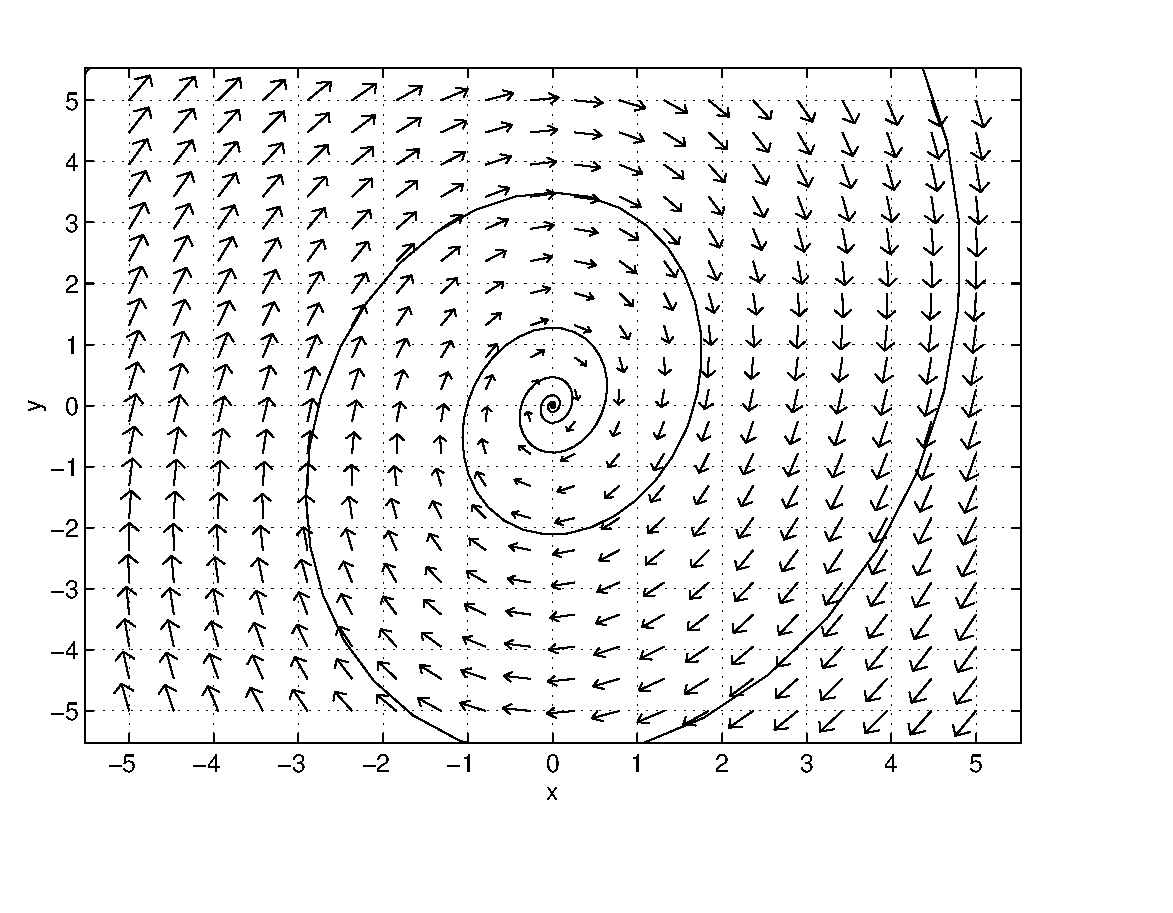
\psfig{file=figures/cmplxfig.eps,width=3.0in}
        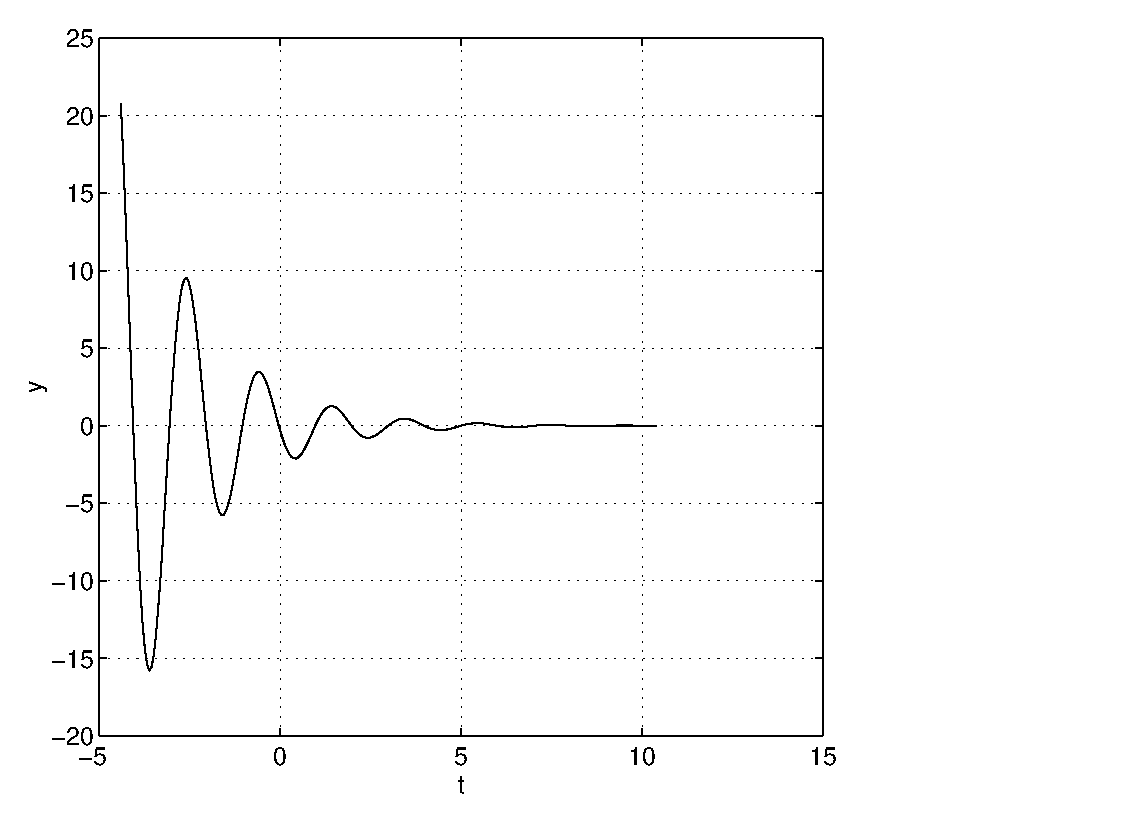
\psfig{file=figures/cmplxtm.eps,width=3.0in}}
        \caption{(Left) Phase plane for \protect\Ref{e:complex2}
              for $x,y\in [-5,5]$.  (Right) Time series $y$ versus $t$
	      of solution}
        \label{rotfig}
\end{figure}




\subsubsection*{Nodal Sinks}
\index{nodal sink}

When the eigenvalues are real and unequal, we get a nodal sink.
For example, consider the differential equation
\begin{eqnarray*}
\dot{x} & = & -x+y \\
\dot{y} & = & -2y
\end{eqnarray*}
whose phase portrait\index{phase!portrait!for a nodal sink} is pictured
in Figure~\ref{F:nodalsink} (left)
along with the time series of one of the solution trajectories (right).
Compare the time series of a solution to a nodal sink equation
with the time series of the spiral sink solution given in
Figure~\ref{rotfig} (right).  Note how the solution asymptotes
to zero rather than oscillating about zero.

\begin{figure}[htb]
           \centerline{%
	   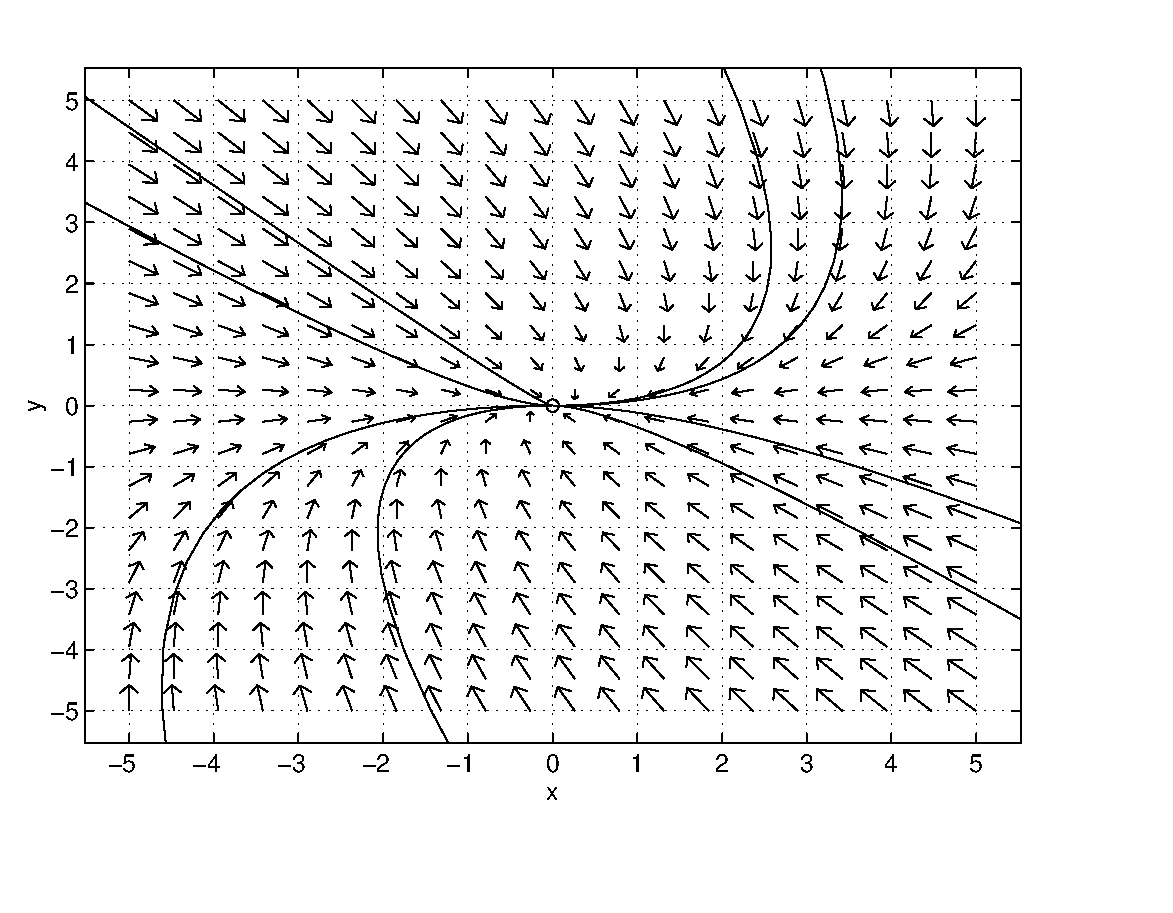
\psfig{file=figures/linnna.eps,width=3.5in}
           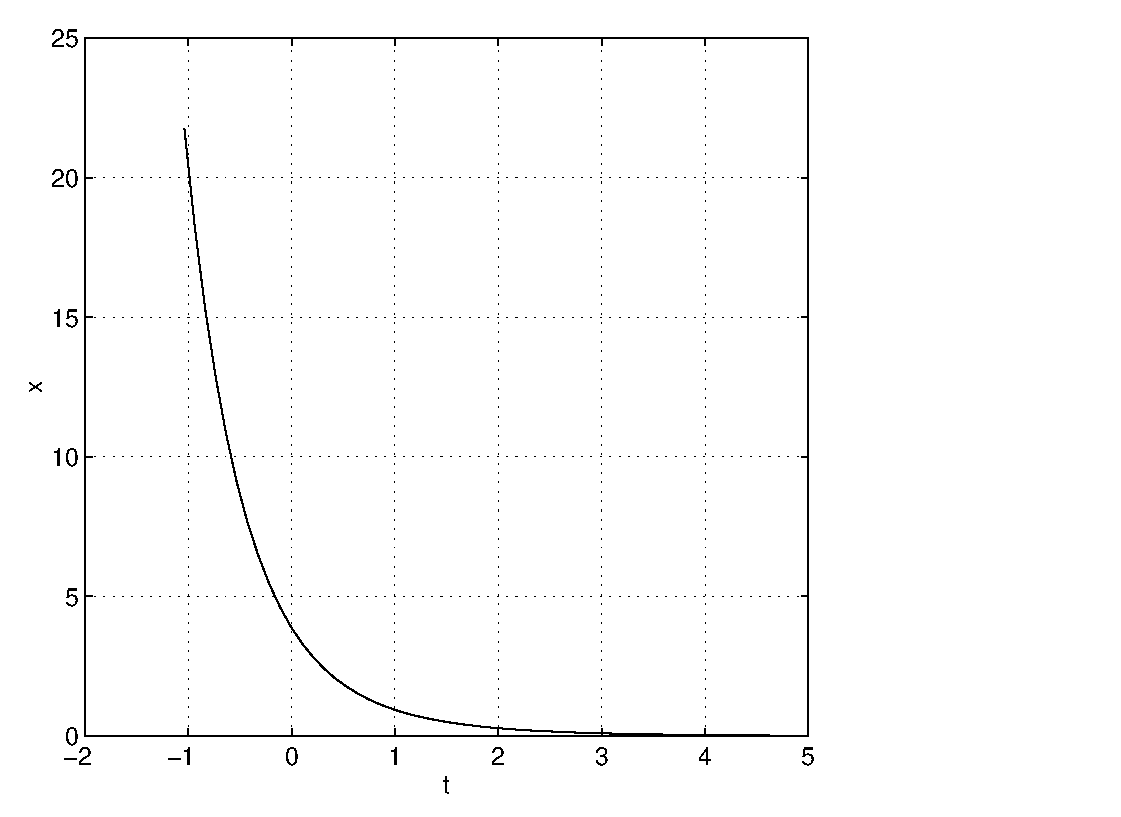
\psfig{file=figures/linnnb.eps,width=3.5in}}
           \caption{(Left) Phase plane of nodal sink.
	(Right) Time series of a typical trajectory.}
           \label{F:nodalsink}
\end{figure}

Moreover, suppose that the eigenvalues are $\lambda_1 < \lambda_2
< 0$.  Then all trajectories approach the origin in forward time
tangent to the eigendirection associated with the eigenvalue
$\lambda_2$.   To verify this point, let $v_1$ and $v_2$ be the
associated eigenvectors.  Then, the general solution has the
form
\[
X(t) = \alpha_1e^{\lambda_1 t}v_1 + \alpha_2e^{\lambda_2 t}v_2
= e^{\lambda_2 t}(\alpha_1e^{(\lambda_1-\lambda_2)t}v_1 + \alpha_2v_2).
\]
Since $\lambda_1-\lambda_2<0$, in forward time $X(t)$ approaches
$e^{\lambda_2 t}\alpha_2v_2$, which is tangent to the $v_2$
eigendirection.  The eigenvalues in our example are $\lambda_1=-2$
and $\lambda_2=-1$, and the eigenvector $v_2$ is just $e_1$.
Indeed, note how trajectories in the phase plane  Figure~\ref{F:nodalsink}
(left) approach the origin tangent to the $x$-axis.

\subsubsection*{Improper Nodes}
\index{improper node}

There are two types of sinks that correspond to coefficient
matrices with real equal eigenvalues: those with one independent
eigenvector --- an {\em improper node\/} --- and those with two independent
eigenvectors --- a {\em focus\/}.

The phase plane\index{phase!portrait!for an improper node}
of an improper node looks like the one pictured in
Figure~\ref{F:degennodal} (left) along with the time series
of one of the solution trajectories (right).  The equation
that we use in this figure is \Ref{e:shearexample}.
Note that trajectories approach the origin tangent to a single
line --- the line generated by the eigenvector.  In this example, the
eigenvector is approximately $(0.32,0.95)$ which generates a line
through the origin of slope approximately equal to $3$.

\begin{figure}[htb]
           \centerline{%
	   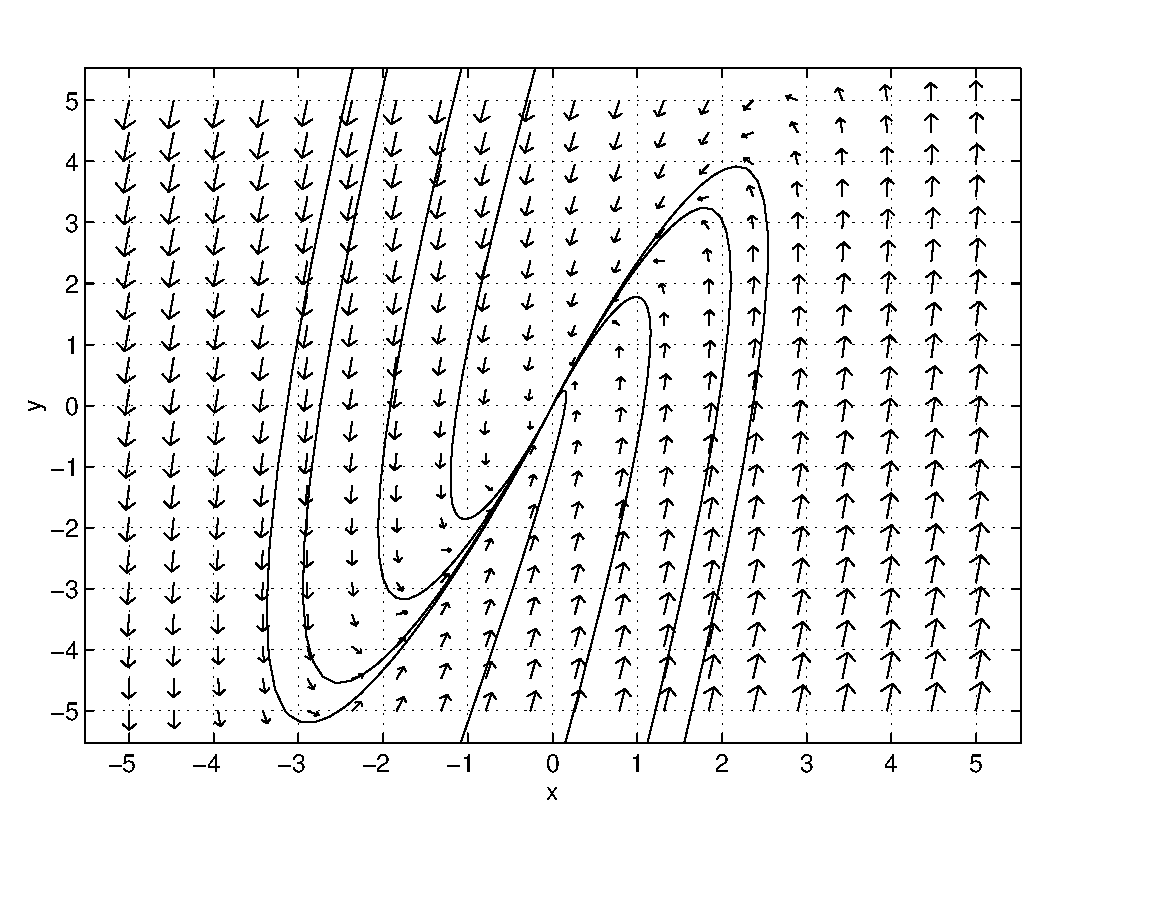
\psfig{file=figures/shearfig.eps,width=3.5in}
           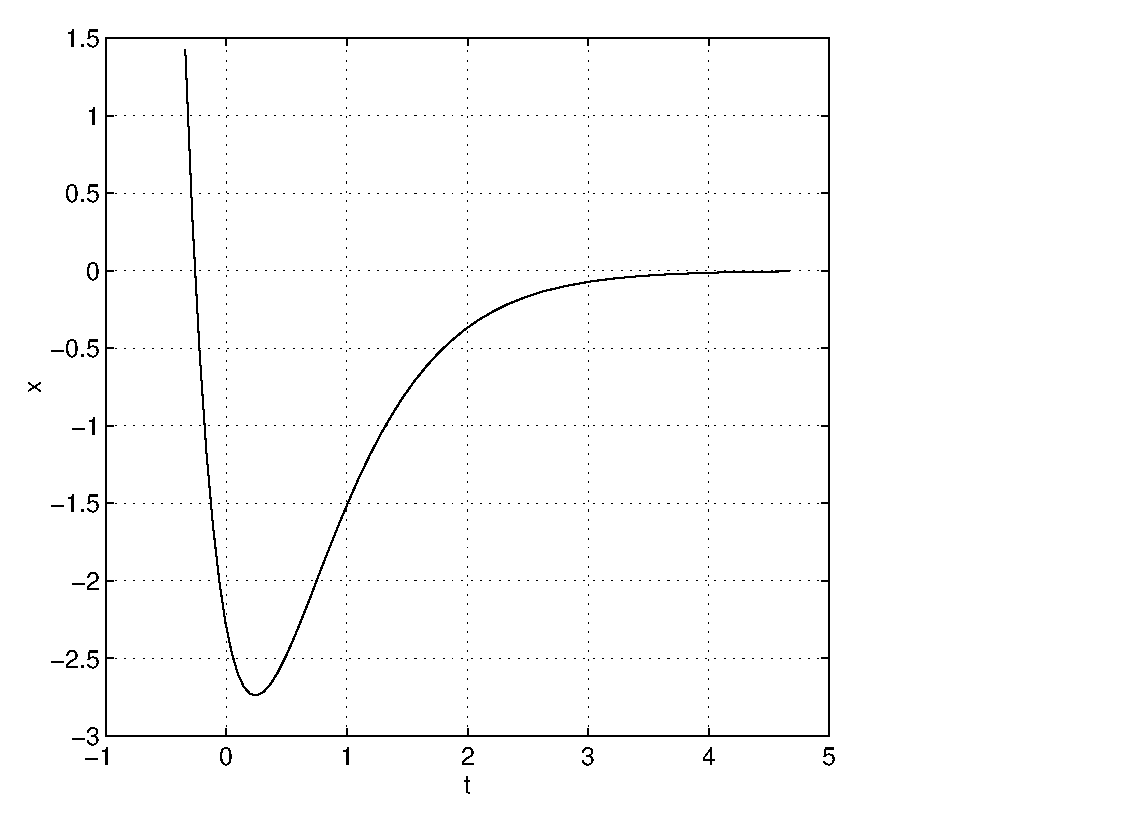
\psfig{file=figures/sheartm.eps,width=3.5in}}
           \caption{(Left) Phase plane of improper nodal sink
	       \protect\Ref{e:shearexample}.  (Right) Time series of
		a trajectory illustrating the transient excursion
		away from zero.}
           \label{F:degennodal}
\end{figure}

Compare the time series of a solution to an improper nodal sink
with either the time series of the spiral sink solution given
in Figure~\ref{rotfig} (right) or the nodal sink given in
Figure~\ref{F:nodalsink} (right).  Note how there is an initial
excursion away from zero followed by a simple asymptote to zero.
This excursion away from zero is typical of nodal sinks. To verify
this point, let $\lambda_1<0$ be the eigenvalue of the coefficient
matrix $C$.  Then the general solution to this equation is:
\[
X(t) = e^{\lambda_1 t}(I_2 + tN)X_0,
\]
where $N = C-\lambda_1 I_2$.
The initial growth in the solution is forced by the $tN$ term.
Eventually, however, exponential decay dominates and the solution
approaches zero.

In addition, solutions approach zero in forward time tangent to
the eigendirection spanned by the eigenvector $v$.  If we choose
a generalized eigenvector $w$ so that $Nw=v$, then we can write the
general solution as
\[
X(t) =  e^{\lambda_1 t}(I_2 + tN)(\alpha v+\beta w) =
e^{\lambda_1 t}\left(\alpha v + \beta w +  t\beta v \right).
\]
For large $t>0$, the solution direction $\alpha v + \beta w + t\beta v$ is
dominated by $t\beta v$, and the trajectory is tangent to the $v$
eigendirection, as claimed.


\subsubsection*{Focuses}
\index{focus}

When the real equal eigenvalues correspond to a coefficient matrix $C$
having two independent eigenvectors, we have a {\em focus\/}.
Lemma~\ref{L:1indeig} of Chapter~\ref{Chap:Planar} states that for a focus,
the matrix $C$ must be a multiple of $I_2$; an example of a focus is the
system of differential equations
\begin{equation}  \label{e:focuseqn}
\begin{array}{rcl}
\dot{x} & = & -0.5x \\
\dot{y} & = & -0.5y.
\end{array}
\end{equation}
The closed form solution to \Ref{e:focuseqn} is just
\[
(x(t),y(t)) = e^{-0.5t}(x_0,y_0).
\]
So solutions remain on straight lines for all time.  The phase
plane\index{phase!portrait!for a focus} for this equation is
pictured in Figure~\ref{F:degennodes}
(left), confirming that solutions stay on lines through the
origin.  Algebraically, the reason for this behavior is that every
line through the origin is an eigendirection.  There are an infinite number
of eigendirections even though there are only two independent eigenvectors.

\begin{figure}[htb]
           \centerline{%
	   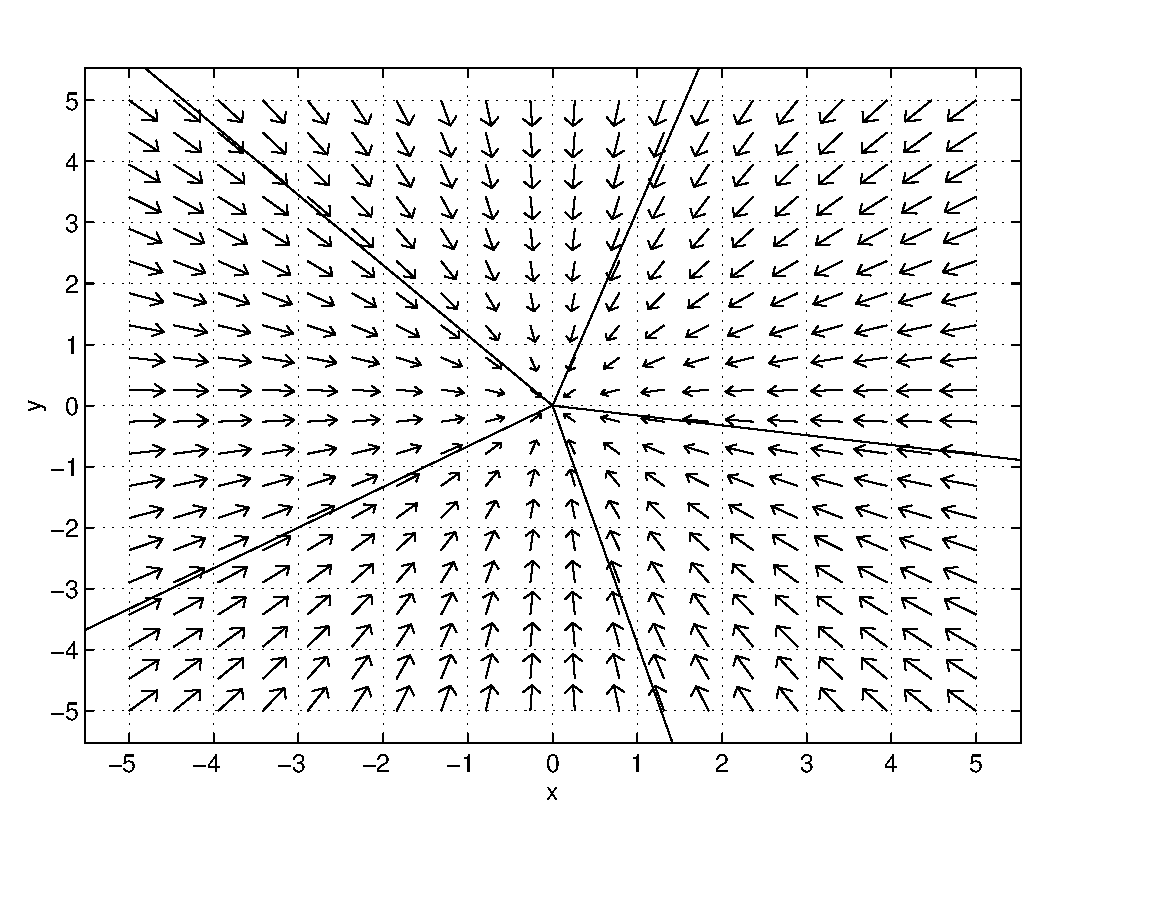
\psfig{file=figures/linfoc.eps,width=3.0in}
           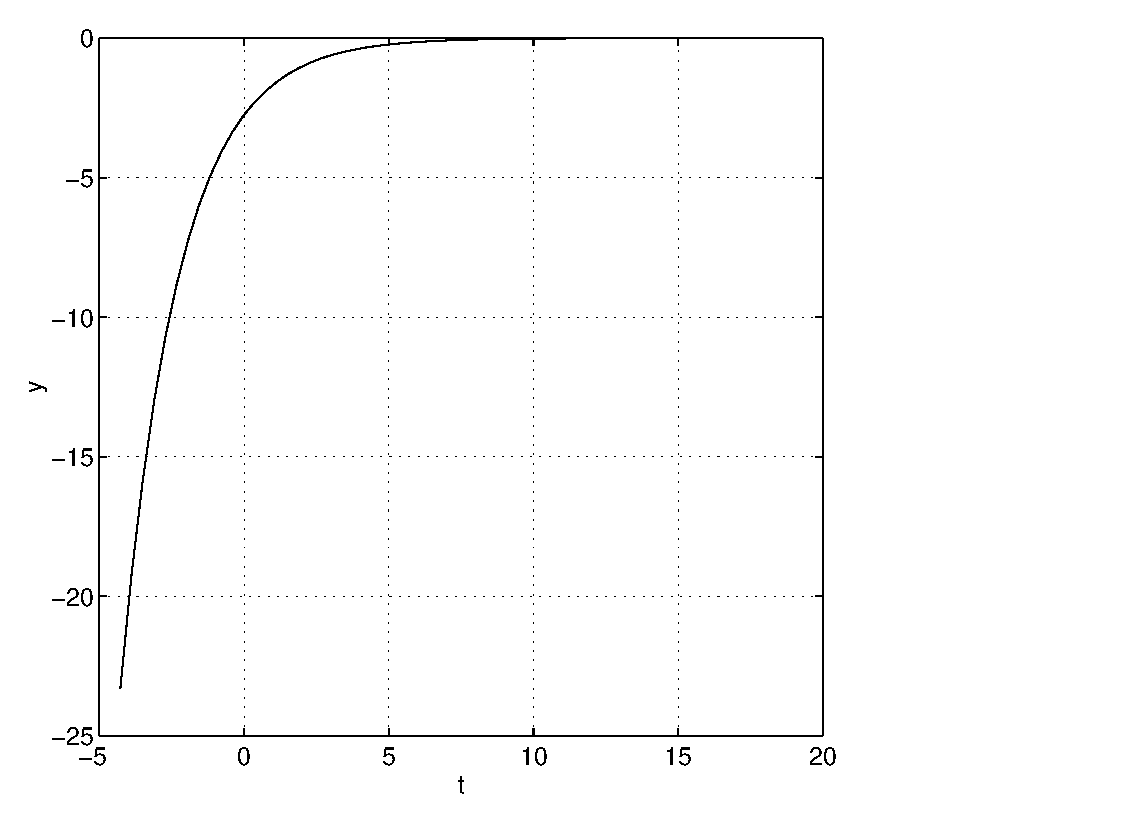
\psfig{file=figures/linfoctm.eps,width=3.0in}}
           \caption{(Left) Phase plane of a focus.
	(Right) Time series of a focus.}
           \label{F:degennodes}
\end{figure}

\subsection*{Hyperbolic Systems}

The simplest linear systems are the sinks, sources, and saddles.
These linear systems all have eigenvalues that are neither zero
nor purely imaginary.  We call the linear system $\dot{X}=CX$
{\em hyperbolic\/} when all eigenvalues of $C$ have nonzero
real parts.  \index{hyperbolic}

Our discussion of phase portraits of hyperbolic linear systems is
summarized in Table~\ref{T:hyperbolic}.  There we reinforce the
observation that the type of phase portrait is determined completely
by the eigenvalues and eigenvectors of the coefficient matrix of the
linear system.

\begin{table}[htb]
\begin{tabular}{|c|c|}
\hline
NAME & EIGENVALUES \\
\hline
saddle    & real and of opposite sign\\
\hline
spiral  sink & complex with negative real part \\
spiral source & complex with positive real part \\
\hline
nodal sink & real, unequal, and negative\\
nodal source & real, unequal, and positive\\
\hline
improper nodal sink & real, equal, negative, and one eigenvector\\
improper nodal source & real, equal, positive, and one eigenvector\\
\hline
focus sink & real, equal, negative, and two independent eigenvectors\\
focus source & real, equal, positive, and two independent eigenvectors\\
\hline
\end{tabular}
\caption{Classification of planar hyperbolic equilibria.}
\label{T:hyperbolic}
\end{table}\index{saddle}\index{sink}\index{source}
\index{nodal sink}\index{nodal source}\index{nodal sink!improper}
\index{nodal source!improper}\index{focus!sink}\index{focus!source}

Another way to determine the type of phase portrait for the
{\em hyperbolic\/} linear system $\dot{X}=CX$ is through the
determinant\index{determinant}, trace\index{trace} and
discriminant\index{discriminant} of $C$. This determination can be made by
answering the following four questions in order.
\begin{itemize}
\item[(Q1)]  {\bf What is the determinant of $C$?}
\[
\det(C) \quad \left\{\begin{array}{ccl}
negative & \Rightarrow & \mbox{The origin is a {\em saddle\/}. Stop.}  \\
zero 	& \Rightarrow & \mbox{The system is not hyperbolic. Stop.}  \\
positive & \Rightarrow & \mbox{Continue.}  \end{array}\right.
\]
\item[(Q2)]  {\bf What is the trace of $C$?}
\[
\trace(C) \quad \left\{\begin{array}{ccl}
positive & \Rightarrow & \mbox{The origin is a {\em source\/}. Continue.}  \\
zero 	& \Rightarrow & \mbox{The system is not hyperbolic. Stop.}  \\
negative & \Rightarrow & \mbox{The origin is a {\em sink\/}. Continue.}
\end{array}\right.
\]
\item[(Q3)]  {\bf What is the discriminant $D$ of $C$?}
\[
D\equiv \trace(C)^2-4\det(C) \quad \left\{\begin{array}{ccl}
negative & \Rightarrow & \mbox{The origin is a {\em spiral\/}. Stop.}  \\
positive & \Rightarrow & \mbox{The origin is a {\em node\/}. Stop.} \\
zero 	& \Rightarrow & \mbox{Continue.}
\end{array}\right.
\]
\item[(Q4)]  {\bf Is $C$ a multiple of $I_2$?}
\[
\left\{\begin{array}{ccl}
no & \Rightarrow & \mbox{The origin is an {\em improper node\/}. Stop.}  \\
yes & \Rightarrow & \mbox{The origin is a {\em focus\/}. Stop.}
\end{array}\right.
\]
\end{itemize}

We now verify that the answers to these four questions do indeed
determine the phase portraits of hyperbolic linear systems.  Recall
from \Ref{e:deteigen} that the determinant is the product of the
eigenvalues.  So if the determinant is negative, then $C$ must have
one negative eigenvalue and one positive eigenvalue, and the origin
is a saddle.  It also follows that $C$ has a zero eigenvalue when
$\det(C)=0$, which contradicts hyperbolicity.  When $\det(C)>0$
either $C$ has two real eigenvalues of the same sign or a complex
conjugate pair of eigenvalues.

Next recall from \Ref{e:treigen} of Section~\ref{S:evchp} that the trace is 
the sum of the 
eigenvalues. Suppose the trace of $C$ is negative.  If the eigenvalues
of $C$ are real, then the two eigenvalues must be negative since they
have the same sign, and the origin is a sink.  If the eigenvalues are
a complex conjugate pair, then the trace is twice the real part of the
eigenvalues.  So again the origin is a sink.  A similar discussion
verifies that the origin is a source when the trace of $C$ is positive.
Note that $\det(C)>0$ and $\trace(C)= 0$ implies that $C$ has purely
imaginary eigenvalues which contradicts the hyperbolicity of $C$.

To understand the conclusions of question (Q3) recall from
Theorem~\ref{eigendist} of Chapter~\ref{chap:SolveOdes} that the 
eigenvalues of $C$ are complex
conjugates when the discriminant $D$ is negative. Hence the origin is
a spiral.  Similarly, if $D>0$, then the eigenvalues of $C$ are real,
and the origin is a node.  Finally, if $D=0$, then the eigenvalues of
$C$ are real and equal.  The origin is an improper node when there is
only one linearly independent eigenvector, and the origin is a focus
when there are two linearly independent eigenvectors.  Moreover, when
a $2\times 2$ matrix has two equal eigenvalues and two linearly
independent eigenvectors, it is a multiple of $I_2$.

See Figure~\ref{F:td} for a classification of phase portrait types
in the determinant-trace plane\index{determinant-trace plane}.

\begin{figure}[htb]
           \centerline{%
           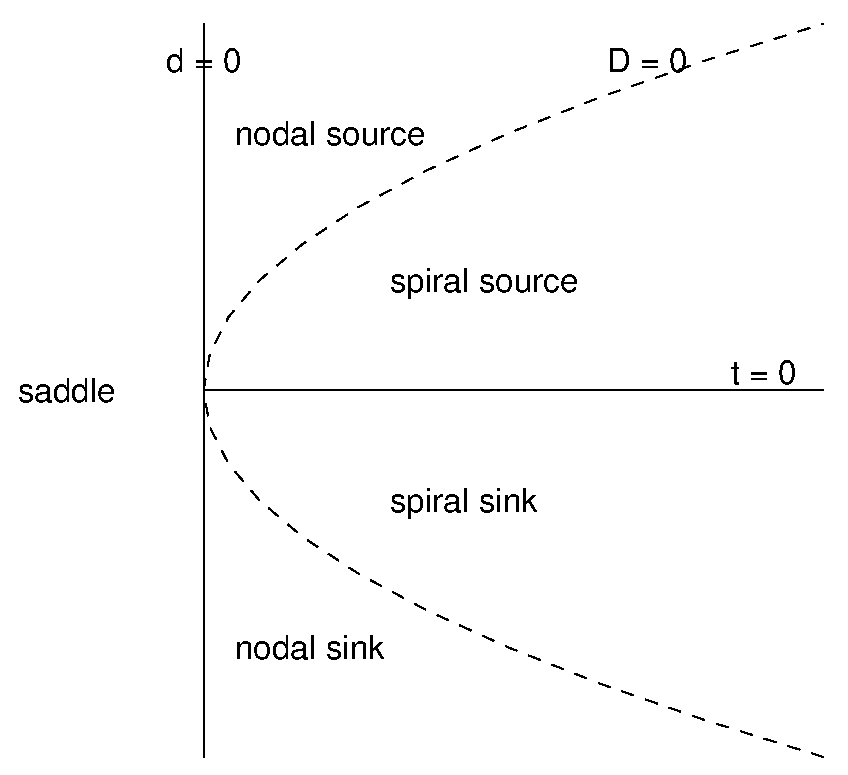
\psfig{file=figures/td.eps,width=3.0in}}
           \caption{Classification of phase portraits in the
		$t$-$d$ plane, where $t$ is the trace, $d$ is the
	determinant, and $D$ is the discriminant.}
           \label{F:td}
\end{figure}

\EXER

\TEXER

\begin{exercise} \label{c6.8.1a}
For the matrix $C$ in Exercise~\ref{E:stabmata} of Section~\ref{S:6.7},
determine the type of phase portrait of $\dot{X}=CX$.
\end{exercise}
\begin{exercise} \label{c6.8.1b}
For the matrix $C$ in Exercise~\ref{E:stabmatb} of Section~\ref{S:6.7}, 
determine the type of phase portrait of $\dot{X}=CX$.
\end{exercise}
\begin{exercise} \label{c6.8.1c}
For the matrix $C$ in Exercise~\ref{E:stabmatc}  of Section~\ref{S:6.7},
determine the type of phase portrait of $\dot{X}=CX$.
\end{exercise}

\noindent In Exercises~\ref{c6.8.2a} -- \ref{c6.8.2d}, find a $2\times 2$
matrix $C$ so that the given statement is satisfied.
\begin{exercise} \label{c6.8.2a}
The differential equation $\dot{X}=CX$ has a saddle at the origin with
unstable orbit in the direction $(2,3)$.
\end{exercise}
\begin{exercise} \label{c6.8.2b}
The differential equation $\dot{X}=CX$ has a spiral sink at the origin
where solutions decay to the origin at rate $\sigma=-0.5$.
\end{exercise}
\begin{exercise} \label{c6.8.2c}
The differential equation $\dot{X}=CX$ has an improper nodal source at the
origin with trajectories approaching the origin tangent to the $y$ axis.
\end{exercise}
\begin{exercise} \label{c6.8.2d}
The differential equation $\dot{X}=CX$ has a nodal sink at the origin with
trajectories approaching the origin tangent to the line $y=x$.
\end{exercise}

\begin{exercise} \label{c6.8.3}
Each picture in Figure~\ref{F:E:timeseries} is the time series of a
solution to a planar system of differential equations of the form
$\dot{X}=CX$.  Describe the eigenvalues of $C$ and determine the type
of planar phase for each of these systems.
\end{exercise}
\begin{figure}[htb]
        \centerline{%
        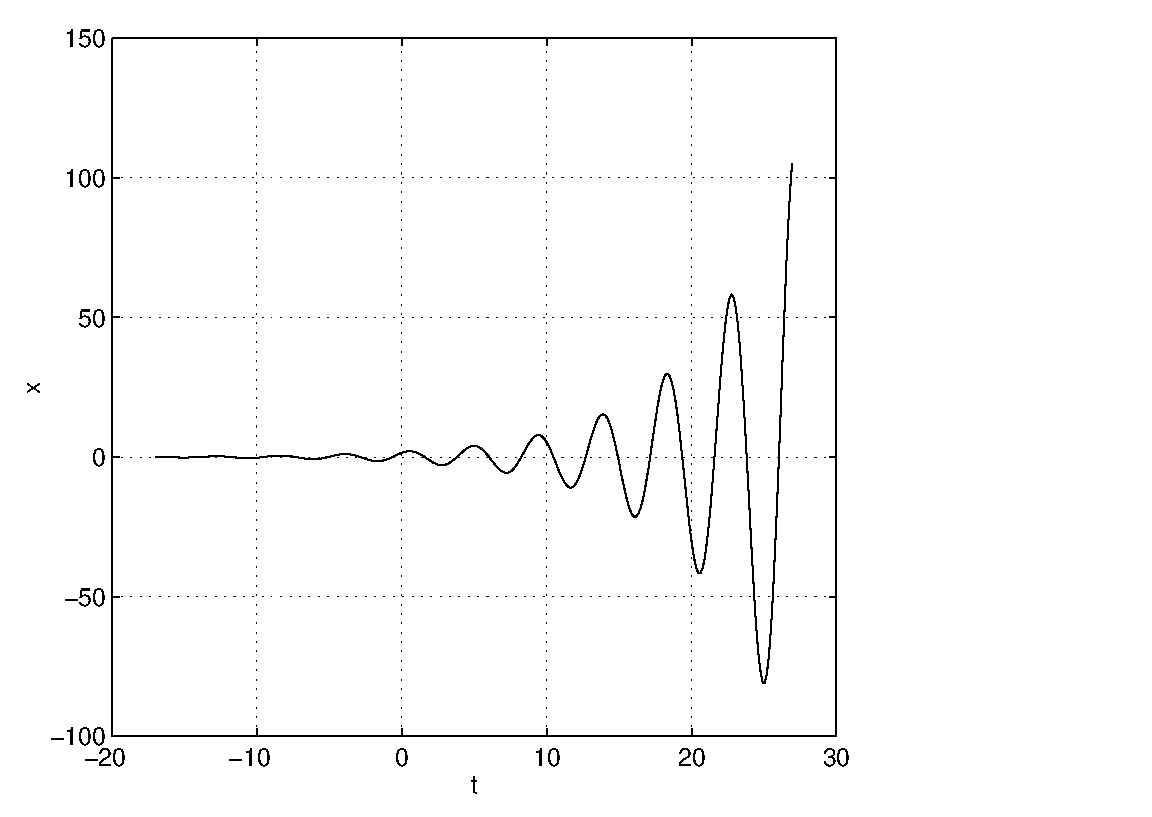
\psfig{file=figures/exspirals.eps,width=3.2in}
        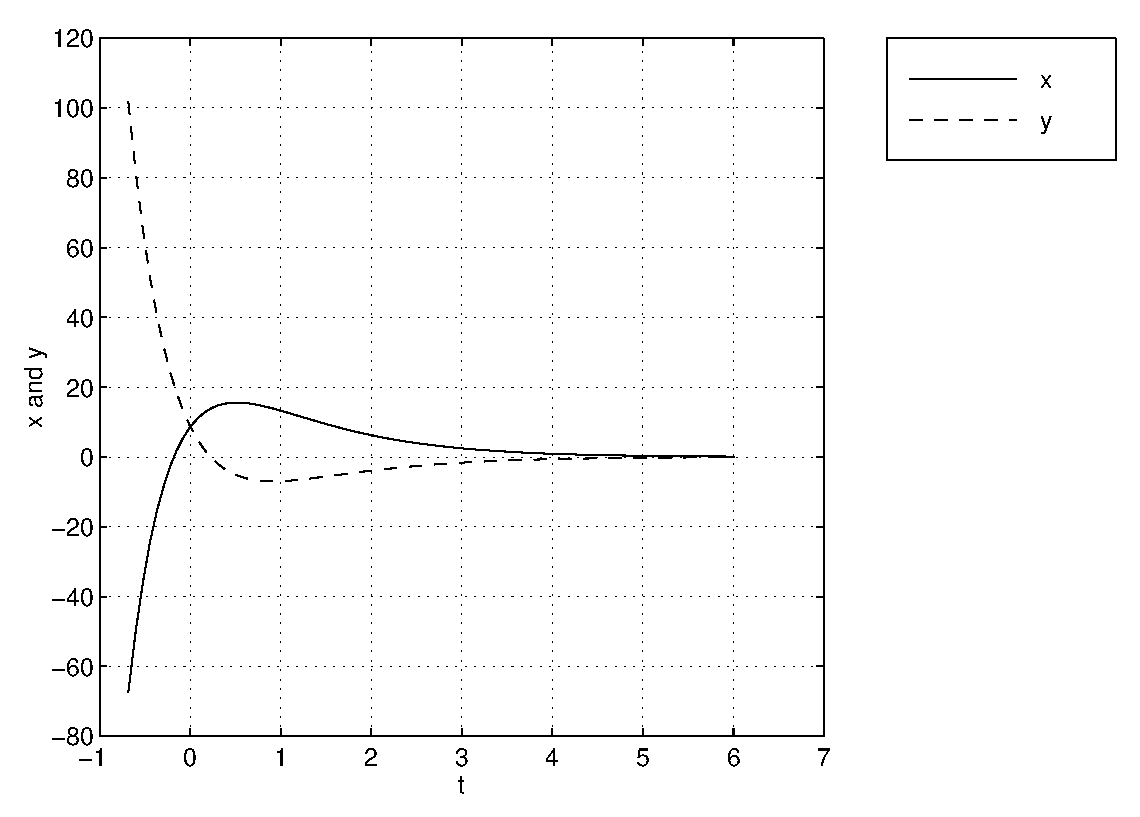
\psfig{file=figures/exsink.eps,width=3.2in}}
	\caption{Time series for planar systems.}
	\label{F:E:timeseries}
\end{figure}


\CEXER

\noindent In Exercises~\ref{c6.8.4a} -- \ref{c6.8.4b}, use {\sf pplane5} to
determine the type of phase portrait for the systems of differential equations
$\dot{X}=CX$ where $C$ is the given matrix.  Based on these computations
answer the following questions:
\begin{itemize}
\item[(a)]  Is the origin asymptotically stable?
\item[(b)]  How many real eigenvectors does the matrix $C$ have?
\end{itemize}
\begin{exercise} \label{c6.8.4a}
$C=\mattwo{\pi}{\sqrt{2}}{-1}{1}$.
\end{exercise}
\begin{exercise} \label{c6.8.4b}
$C=\mattwo{4}{1}{6}{-1}$.
\end{exercise}


\Section{Phase Portraits of Nonhyperbolic Systems} \label{S:6.9}

A linear constant coefficient system $\dot{X}=CX$ is not hyperbolic
\index{nonhyperbolic}
when either $C$ has a zero eigenvalue ($\det(C)=0$) or when $C$ has
purely imaginary eigenvalues ($\det(C)>0$ and $\trace(C)=0$).  These
special cases are indicated by bold lines in Figure~\ref{F:td}.

There are four types of nonhyperbolic planar systems.  There are:
\begin{enumerate}
\item	the {\em center}\index{center} --- nonzero purely imaginary
eigenvalues,
\item	the {\em saddle-node\/}\index{saddle-node} --- a single
zero eigenvalue,
\item	the {\em shear\/}\index{shear} --- a double zero eigenvalue;
one  independent eigenvector, and
\item	the zero matrix itself.
\end{enumerate}
The dynamics in the last case are very easy to describe --- all solutions
are equilibria and solutions remain at the initial point for all time.

\subsubsection*{Centers}

There is a new kind of solution that occurs only in centers --- the time
periodic solution\index{periodic solution} --- as we now explain.
In Chapter~\ref{Chap:Planar},
Theorem~\ref{T:putinform} we showed that when the $2\times 2$
matrix $C$ has purely eigenvalues $\pm i\tau$ with $\tau\neq 0$, then $C$
is similar to the matrix
\[
B =   \mattwo{0}{-\tau}{\tau}{0}.
\]
In Table~\ref{T:3sys}(b) we showed that solutions to $\dot{X}=BX$ are
\[
X(t) = \mattwo{\cos(\tau t)}{-\sin(\tau t)}{\sin(\tau t)}{\cos(\tau t)}X_0
=R_{\tau t}X_0,
\]
where $X_0$ is the vector of initial conditions and $R_{\tau t}$ is a
rotation matrix (recall \Ref{e:rotmat} of Chapter~\ref{chap:matrices}).

Note that every solution to $\dot{X}=BX$ traverses a circle around the
origin as $R_{\tau t}$ rotates the plane counterclockwise through the angle
$\tau t$.  As an example, we graph\index{phase!portrait!for a center}
a solution to $\dot{X}=BX$ and its time
series in Figure~\ref{F:center} when $\tau=3$.  All centers have nonzero
trajectories that are either ellipses\index{ellipse} or circles, and
those centers that do
not have the form of $B$ typically produce ellipses as solutions.  See
Exercise~\ref{E:notcircles}.

\begin{figure}[htb]
     \centerline{%
     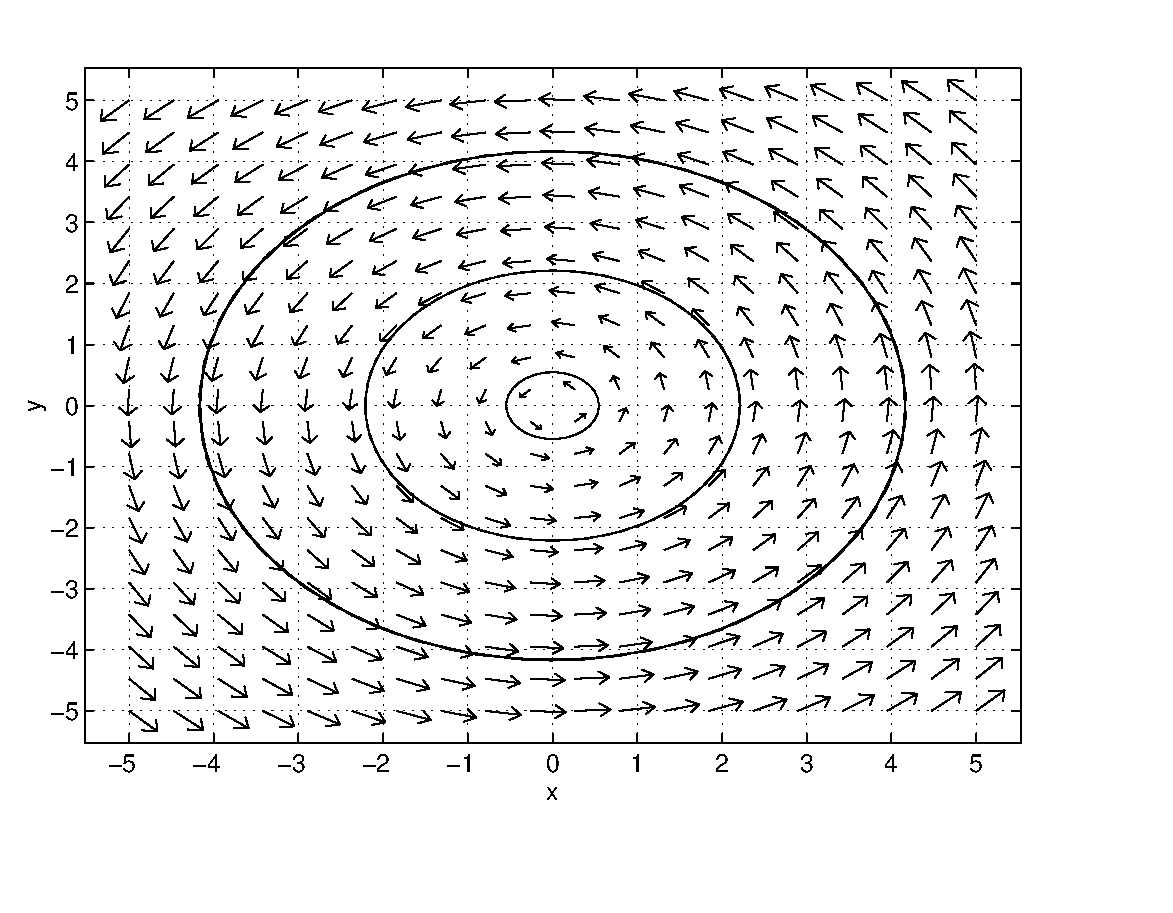
\psfig{file=figures/center.eps,width=2.2in}
     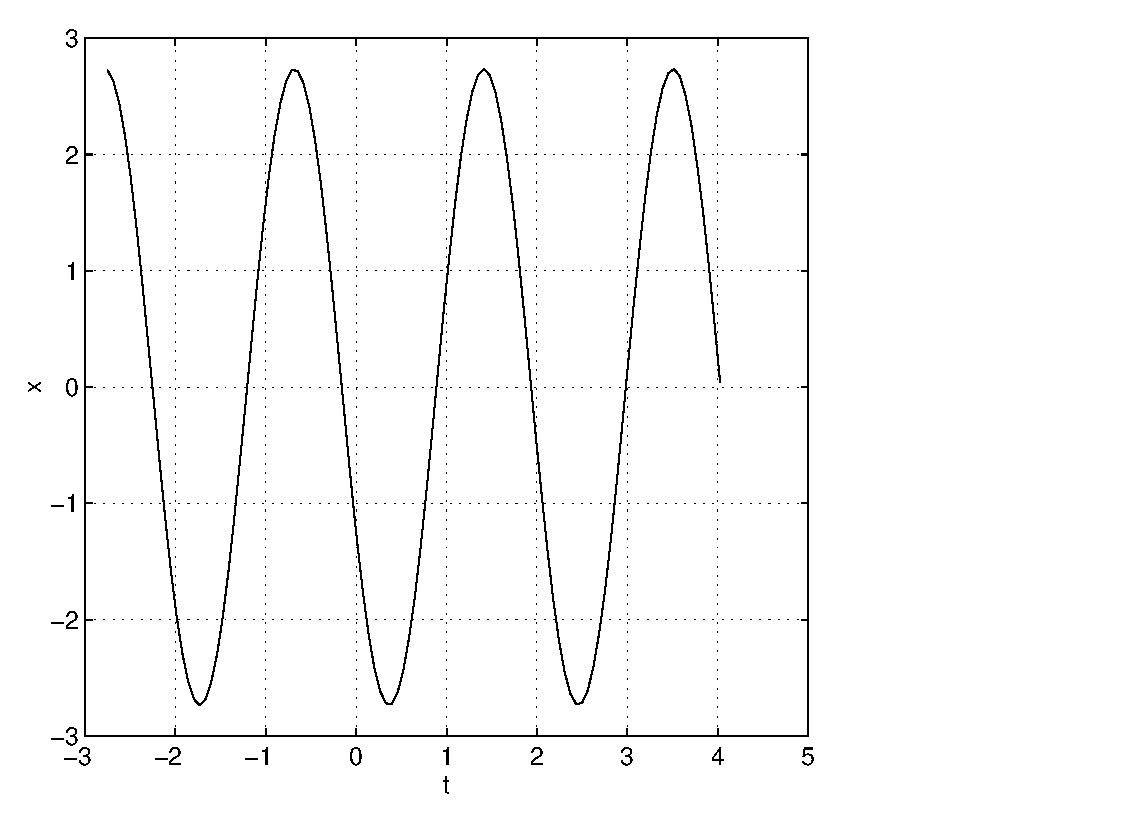
\psfig{file=figures/centerts.eps,width=2.2in}}
     \caption{(Left) Solutions to $\dot{X}=BX$ for $\tau=3$.
	(Right) Time series of a solution illustrating time periodicity.}
     \label{F:center}
\end{figure}

It is instructive to see how solutions change when the real part of the
eigenvalue traverses through zero.  Suppose that $C$ has eigenvalues
$\sigma\pm i\tau$ and is in normal form
\[
C = \mattwo{\sigma}{-\tau}{\tau}{\sigma}.
\]
We illustrate this change by graphing the time series (of both $x$ and $y$
versus $t$) in Figure~\ref{F:spiraling} with $\tau=3$ and $\sigma=-1,0,1$,
respectively. Note that when $\sigma<0$ the time series oscillate about zero
but also damp down to zero, while when $\sigma>0$ the time series oscillate
and diverge.  When $\sigma = 0$, there is an exact balance leading to time
periodic solutions.

\begin{figure}[htb]
     \centerline{%
     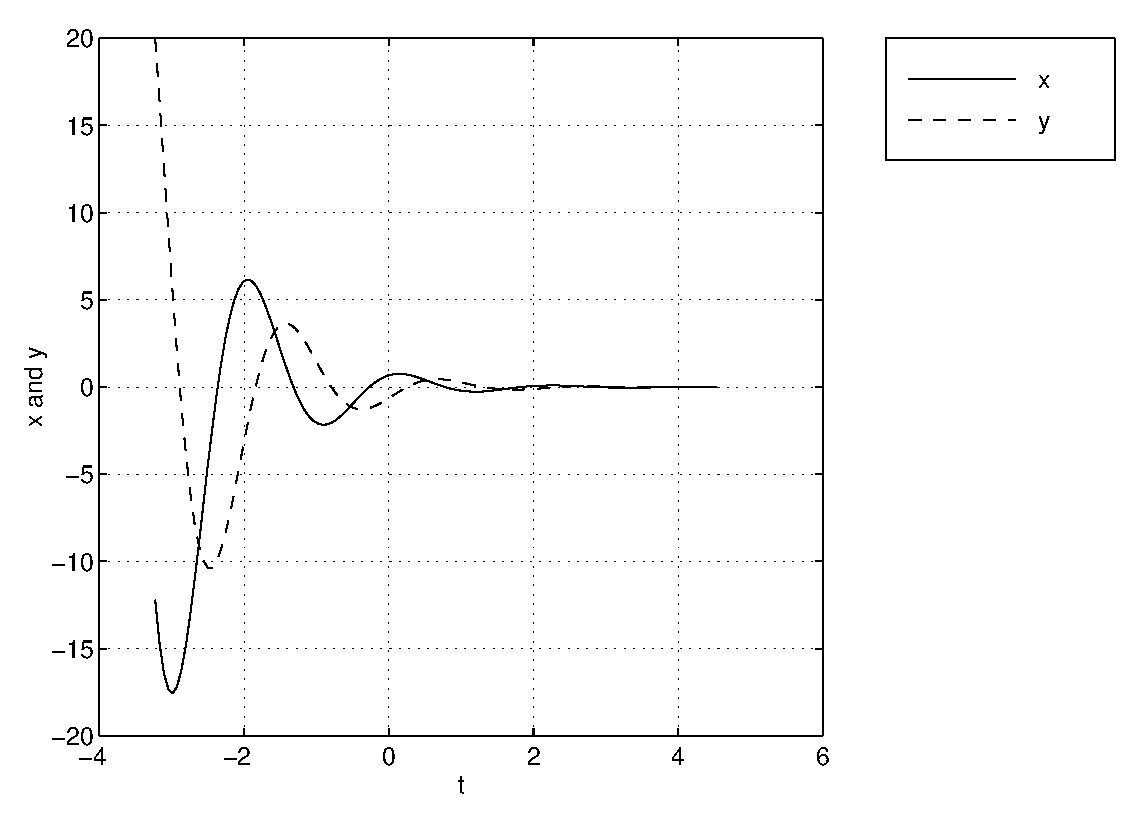
\psfig{file=figures/spn1.eps,width=2.2in}
     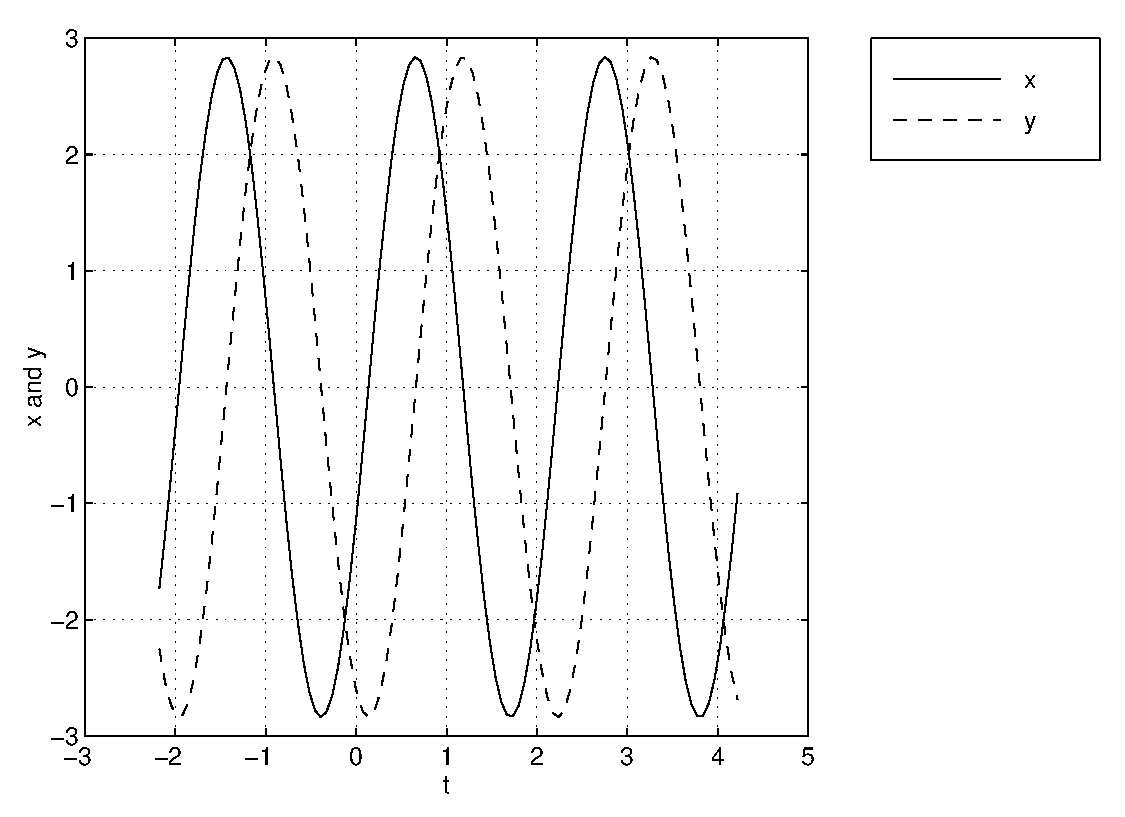
\psfig{file=figures/sp0.eps,width=2.2in}
     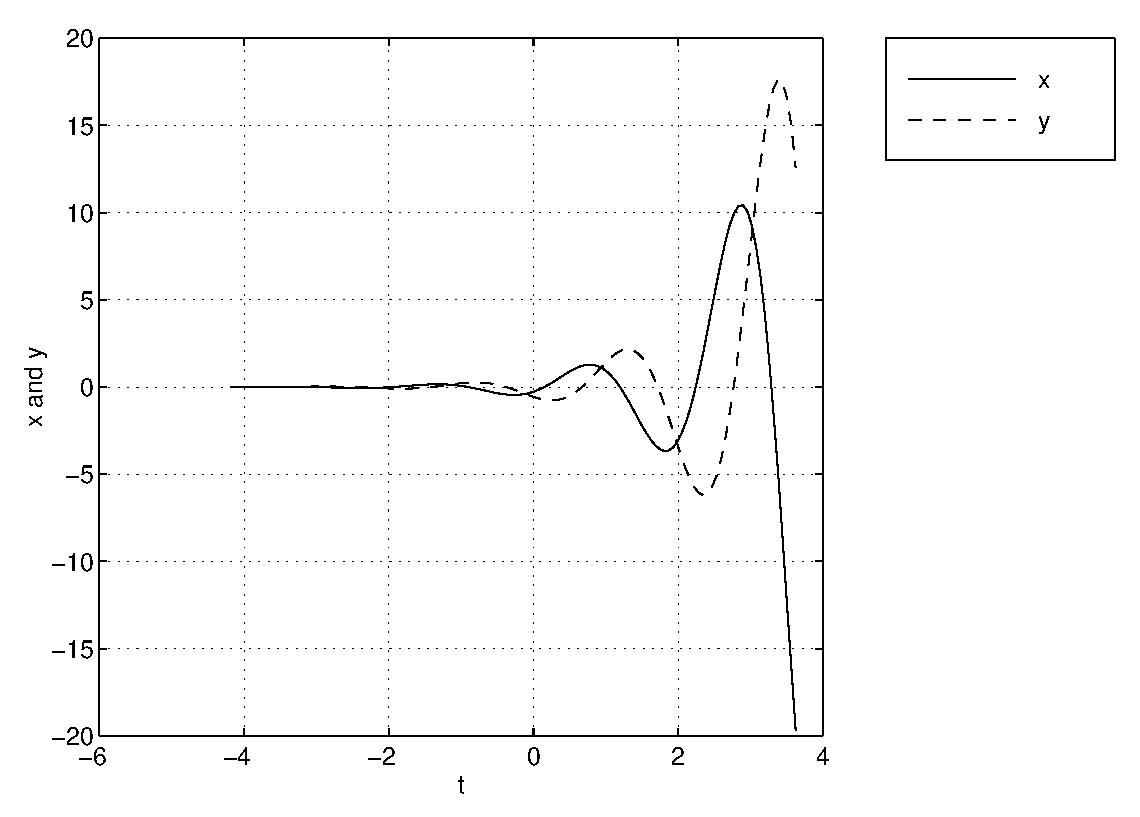
\psfig{file=figures/sp1.eps,width=2.2in}}
     \caption{Solutions of $\dot{X}=BX$ for $\tau=3$ and $\sigma=-1,0,1$.}
     \label{F:spiraling}
\end{figure}

\subsubsection*{Saddle Nodes}

When the determinant of a matrix $C$ is zero, then $C$ must have a zero
eigenvalue.  The simplest way for $\det(C)$ to be zero is for $C$ to have a
single zero eigenvalue.  In this case we call the origin a {\em saddle node}.

So the eigenvalues of a saddle node are $\lambda_1=0$ and $\lambda_2\neq 0$.
For simplicity of discussion, we assume that $\lambda_2<0$.  Let $v_1$ and
$v_2$ be the associated eigenvectors.  Since $Cv_1=0$, it follows that saddle
nodes have a line of equilibria\index{line of equilibria}
$X(t)=\alpha_1v_1$ for every scalar $\alpha_1$.

There is also a solution $X(t)=e^{\lambda_2 t}v_2$ that converges to the
origin in forward time (since $\lambda_2<0$).  The general solution to this
system is
\[
X(t) = \alpha_1 v_1 + \alpha_2 e^{\lambda_2 t}v_2,
\]
for scalars $\alpha_1$ and $\alpha_2$.  Since $\lambda_2<0$ this solution
converges on the equilibrium $\alpha_1 v_1$ in forward time.  Moreover,
the trajectory for any solution stays for all time on the line parallel
to the vector $v_2$.  The phase portrait\index{phase!portrait!for a saddle
node}
for the system
\begin{equation}  \label{e:10ev}
\frac{dX}{dt} = \mattwo{-2}{4}{1}{-2} X
\end{equation}
is shown in Figure~\ref{F:10ev} (left) along with the time series
of a solution (right).  Note how the time series (of $x$ versus $t$)
asymptotes onto the $x$ coordinate of an equilibrium.

\begin{figure}[htb]
     \centerline{%
     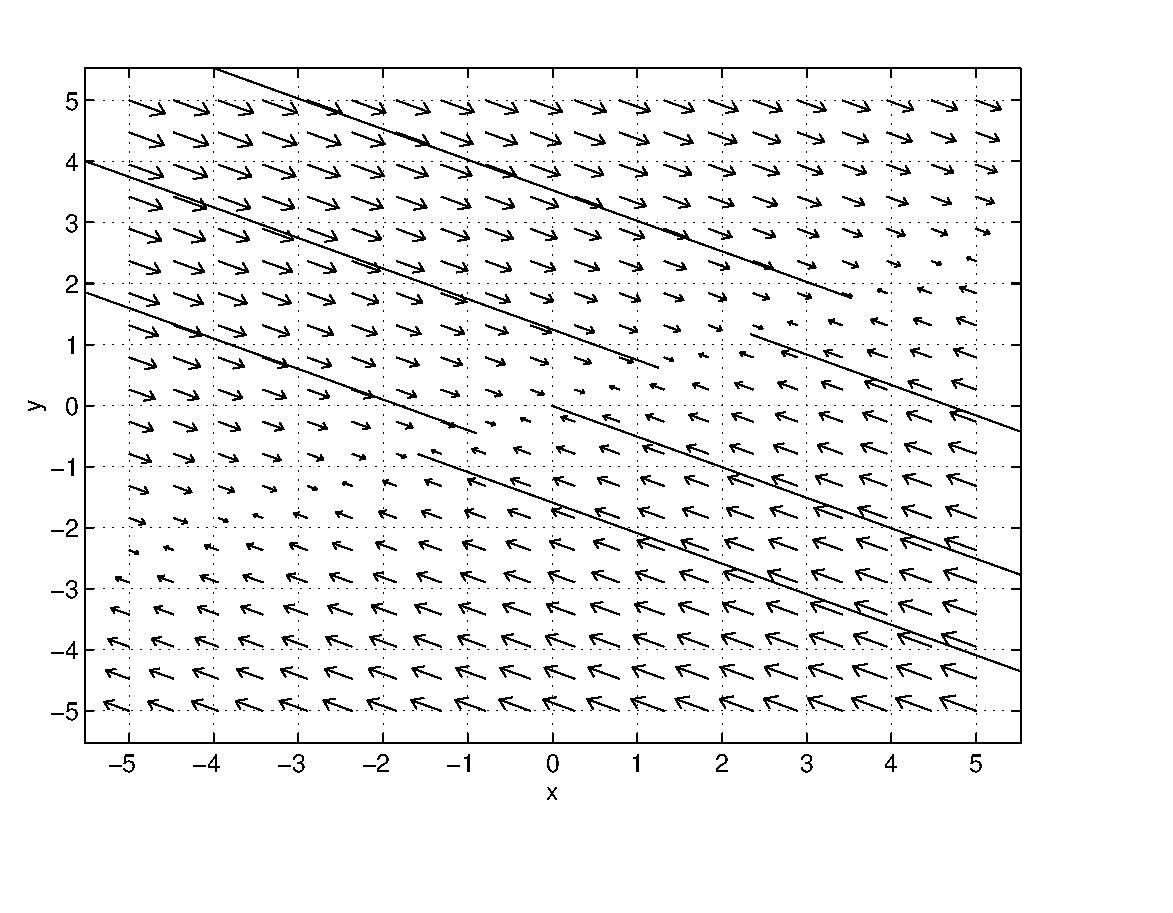
\psfig{file=figures/z1ev.eps,width=2.2in}
     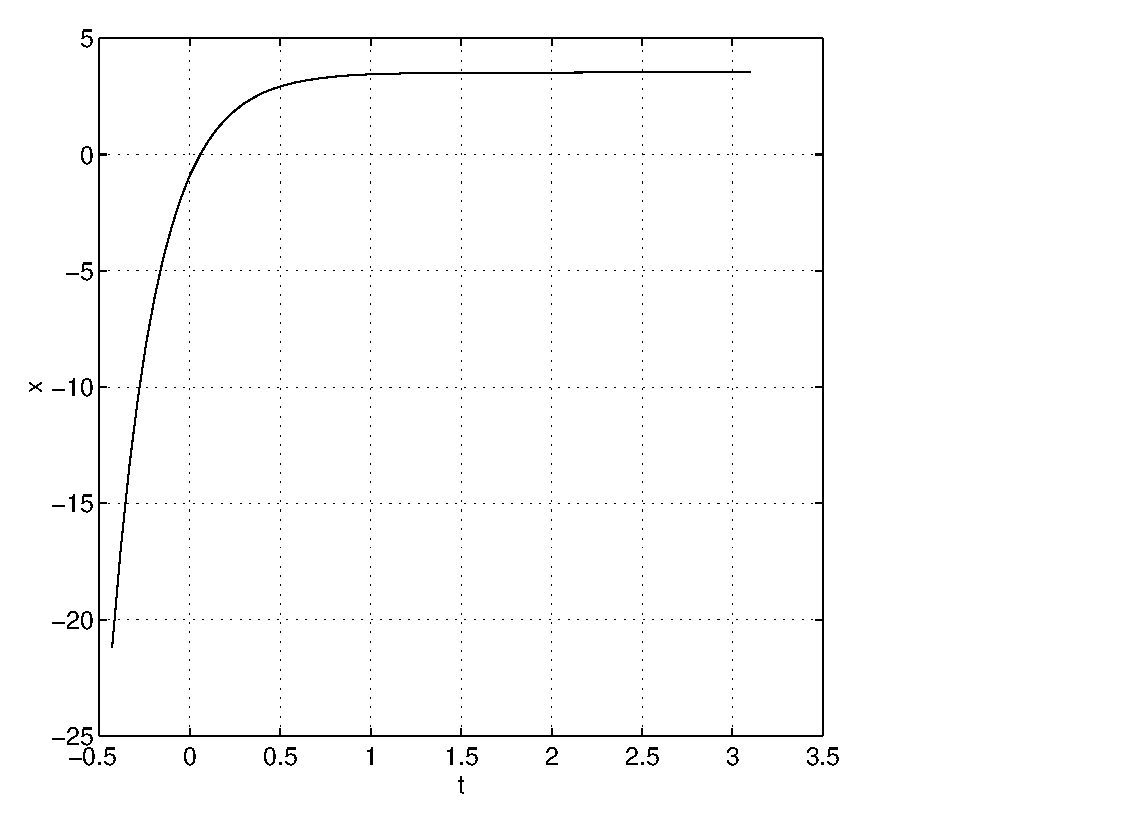
\psfig{file=figures/z1evts.eps,width=2.2in}}
     \caption{(Left) Phase portrait of \protect\Ref{e:10ev}.
	(Right) Time series of a solution.}
     \label{F:10ev}
\end{figure}

The saddle-node\index{saddle-node} is a
nonhyperbolic equilibrium\index{equilibrium!nonhyperbolic}
that sits between
the hyperbolic saddle and the hyperbolic node (either the nodal
sink or the nodal source), just as the center\index{center} sits
between the hyperbolic spiral source and the hyperbolic spiral sink.  To
illustrate this point we show three time series in
Figure~\ref{F:saddlenodebif} for the system
\begin{equation}  \label{e:saddlenodebif}
\frac{dX}{dt}  =  \mattwo{\mu}{0}{0}{-1}X
\end{equation}
when $\mu<0$, $\mu=0$, and $\mu>0$.  See how the $y$ time series
decays exponentially to zero in forward time in each case.  But
the $x$ time series converges to zero when $\mu<0$ and grows
exponentially when $\mu>0$.  Finally, when $\mu=0$ the $x$ time
series is constant.

\begin{figure}[htb]
     \centerline{%
     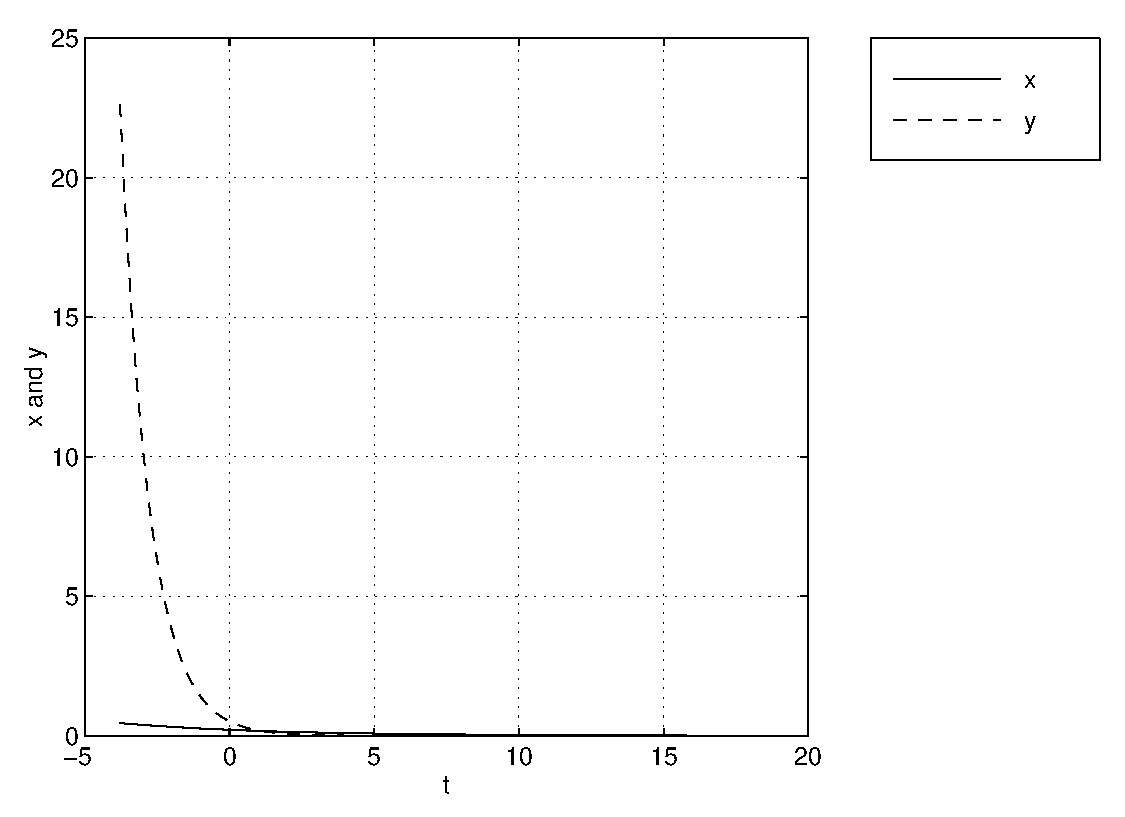
\psfig{file=figures/snn1.eps,width=2.2in}
     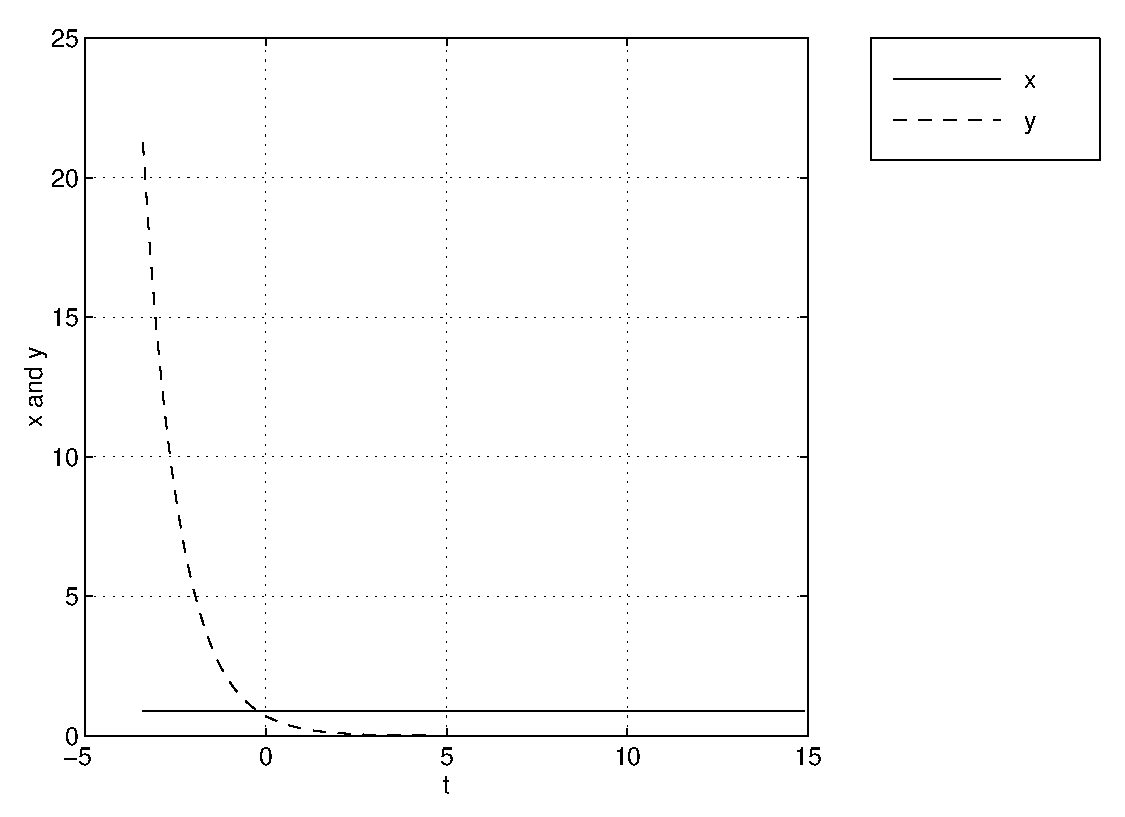
\psfig{file=figures/sn0.eps,width=2.2in}
     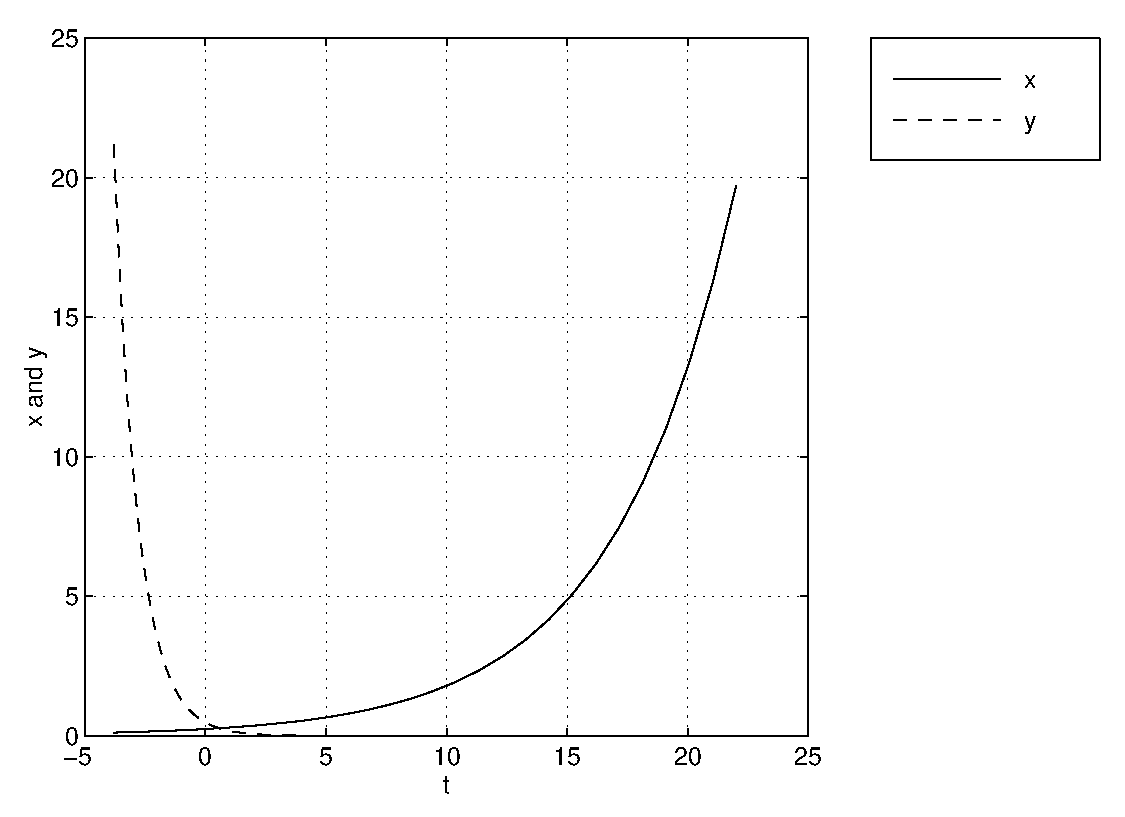
\psfig{file=figures/snp1.eps,width=2.2in}}
     \caption{Time series for solutions of \protect\Ref{e:saddlenodebif}
	when $\mu=-0.2,0,0.2$.}
     \label{F:saddlenodebif}
\end{figure}


\subsubsection*{Shears}
\index{shear}

The last example of a nonhyperbolic system occurs when the matrix $C$
has two zero eigenvalues --- but only one linearly independent
eigenvector.  In this case we call the origin a {\em shear\/}.  After a
similarity transformation such a system is
\begin{equation}  \label{e:00}
\frac{dX}{dt} = \mattwo{0}{1}{0}{0} X
\end{equation}
The solution is
\[
(x(t),y(t)) = (x_0+y_0t,y_0).
\]
Thus solutions move along lines parallel to the $x$ axis through
the point $(x_0,y_0)$ with speed $y_0$.  These trajectories move
to the right when $y_0>0$ and to the left when $y_0<0$.

\EXER

\TEXER

\noindent In Exercises~\ref{c6.9.1a} -- \ref{c6.9.1b}, find a $2\times 2$
matrix $C$ so that the differential equation $\dot{X}=CX$ satisfies the
given condition.
\begin{exercise} \label{c6.9.1a}
The origin is a center.
\end{exercise}
\begin{exercise} \label{c6.9.1b}
The origin is a saddle-node with equilibria on the line generated by the
vector $(-1,2)$.
\end{exercise}

\begin{exercise} \label{c6.9.2}
Recall from Chapter~\ref{Chap:Planar}, \Ref{ex:uspring} that the undamped
spring equation is $\frac{d^2x}{dt^2} + \kappa x = 0$, where $\kappa>0$.
\begin{itemize}
\item[(a)]   As a first order system this equation is:
\begin{eqnarray*}
\dot{x} & = & y \\
\dot{y} & = & -\kappa x.
\end{eqnarray*}
Sketch the phase portrait of this equation.
\item[(b)]  The damped spring equation, written as a first order system, is:
\begin{eqnarray*}
\dot{x} & = & y \\
\dot{y} & = & -\kappa x-\sigma y,
\end{eqnarray*}
where $\sigma>0$ is the damping.  Sketch the phase portrait of this equation.
\end{itemize}
\end{exercise}

\noindent In Exercises~\ref{E:PPa} -- \ref{E:PPe}, consider the four pictures
in Figure~\ref{F:PP}.  Each picture is a phase portrait of a system of
differential equations $\dot{X}=CX$ where $C$ is a $2\times 2$ matrix.  Answer
the given question for each of these phase portraits.
\begin{exercise}  \label{E:PPa}
What is the name of the type of equilibrium at the origin?
\end{exercise}
\begin{exercise}  \label{E:PPb}
Is the origin asymptotically stable?
\end{exercise}
\begin{exercise}  \label{E:PPc}
Is ${\rm trace}(C)$ positive, negative, or zero?
\end{exercise}
\begin{exercise}  \label{E:PPd}
Is $\det(C)$ positive, negative, or zero?
\end{exercise}
\begin{exercise}  \label{E:PPe}
Is ${\rm discriminant}(C)$ positive, negative, or zero?
\end{exercise}

\begin{figure}[htb]
\centerline{(A) \hspace{2.7in} (B)}
           \centerline{%
           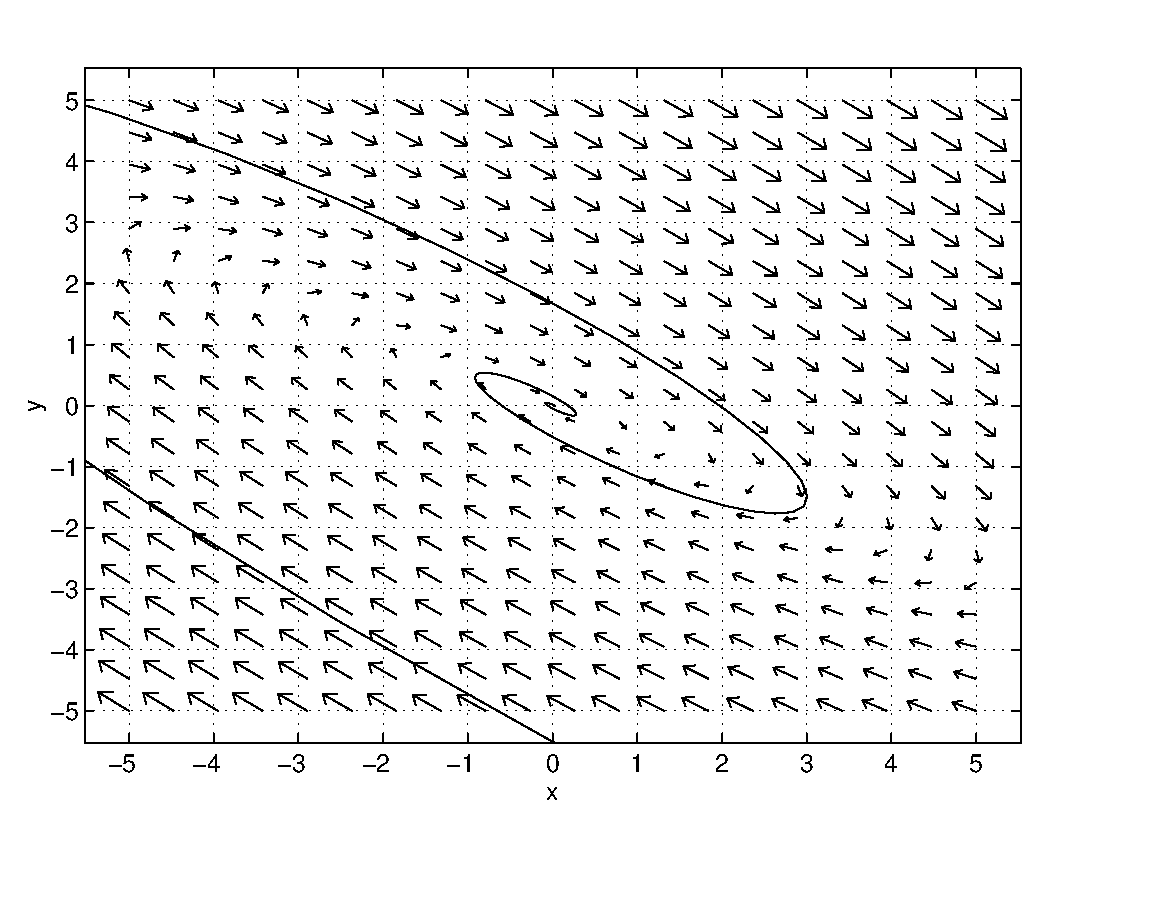
\psfig{file=figures/e2B.eps,width=3.0in}
           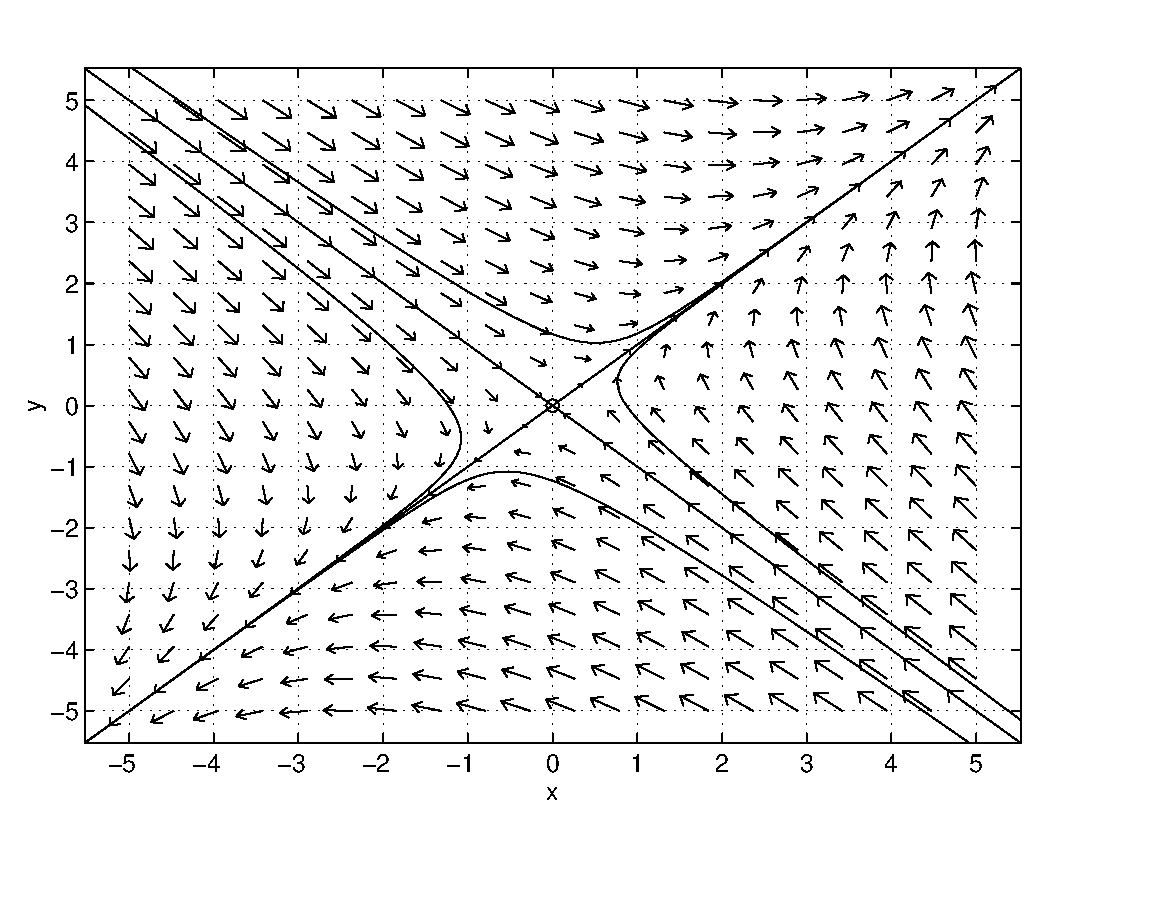
\psfig{file=figures/e2C.eps,width=3.0in}}
\centerline{(C) \hspace{2.7in} (D)}
           \centerline{%
           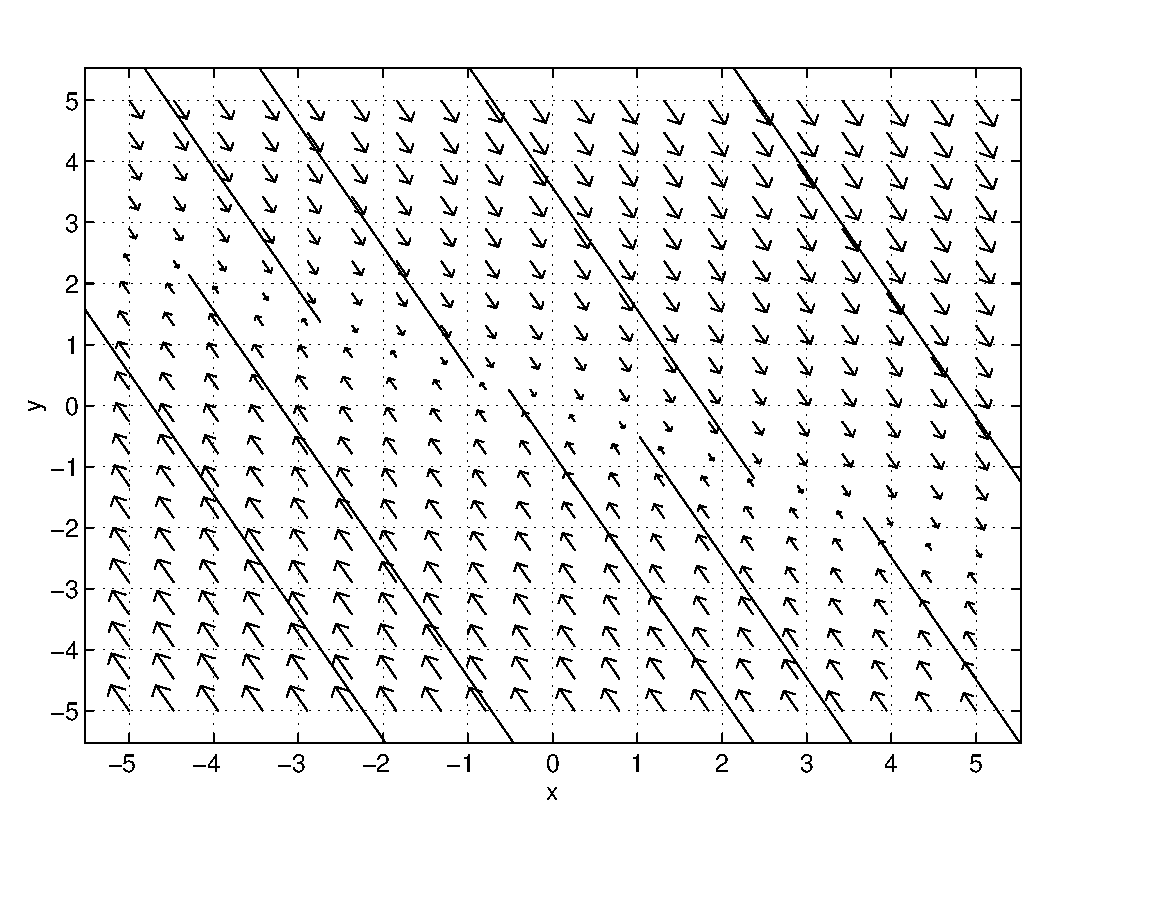
\psfig{file=figures/e2A.eps,width=3.0in}
           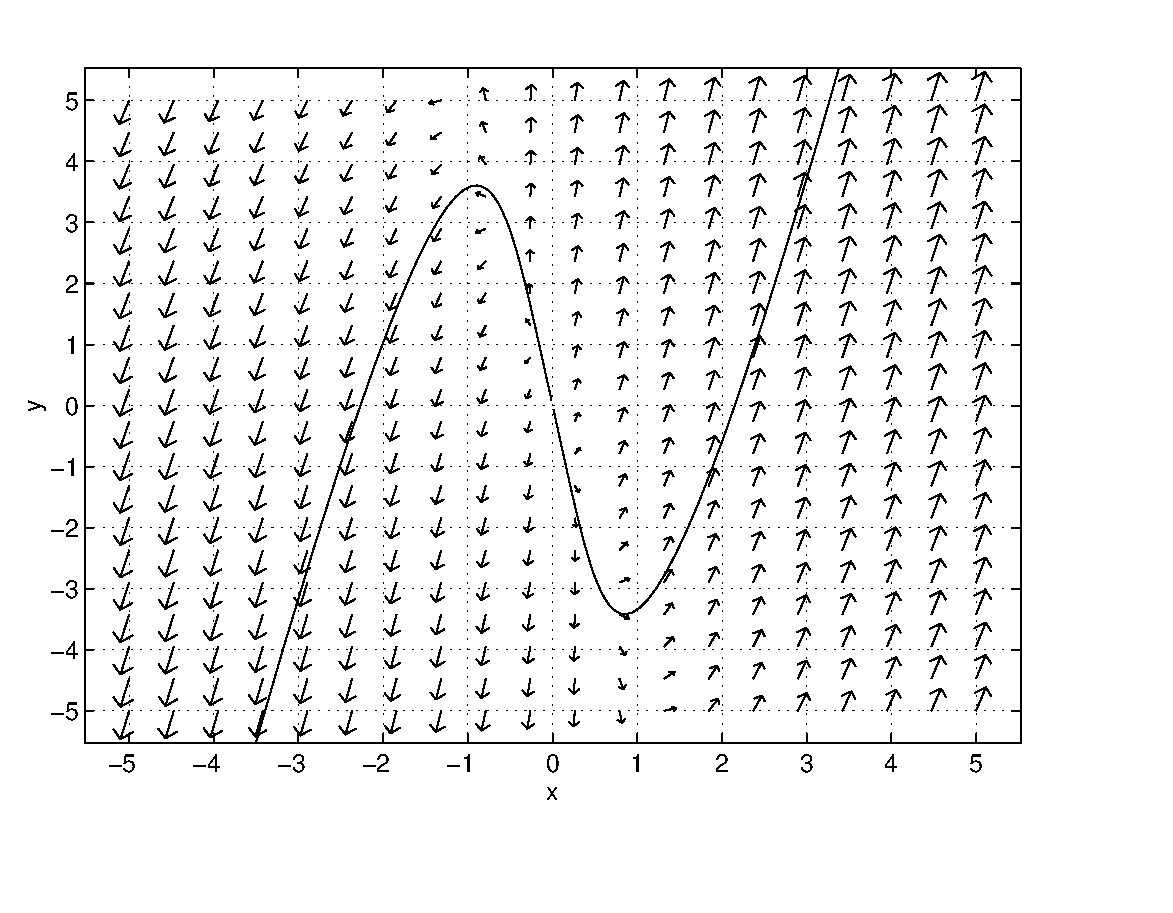
\psfig{file=figures/e2D.eps,width=3.0in}}
\caption{Phase portraits for planar linear systems in
Exercises~\protect\ref{E:PPa} -- \protect\ref{E:PPe}}
\label{F:PP}
\end{figure}

\noindent In Exercises~\ref{E:PQa} -- \ref{E:PQg}, consider the system of
differential equations $\dot{X}=CX$ where $C$ is the given matrix.  For each
system determine whether the origin is hyperbolic or not and the type of
equilibrium at the origin (spiral sink, center, etc.).
\begin{exercise}  \label{E:PQa}
$C = \mattwo{1}{-1}{2}{1}$.
\end{exercise}
\begin{exercise}  \label{E:PQb}
$C = \mattwo{1}{1}{-1}{1}$.
\end{exercise}
\begin{exercise}  \label{E:PQc}
$C = \mattwo{3}{-1}{1}{1}$.
\end{exercise}
\begin{exercise}  \label{E:PQd}
$C = \mattwo{1}{1}{1}{1}$.
\end{exercise}
\begin{exercise}  \label{E:PQe}
$C = \mattwo{2}{-2}{4}{-2}$.
\end{exercise}
\begin{exercise}  \label{E:PQf}
$C = \mattwo{2}{2}{-2}{-2}$.
\end{exercise}
\begin{exercise}  \label{E:PQg}
$C = \mattwo{1}{1}{4}{1}$.
\end{exercise}

\CEXER

\begin{exercise}  \label{E:notcircles}
Consider the system of differential equations $\dot{X}=CX$ where
$C=\mattwo{2}{-10}{1}{-2}$.  By hand show that this system is a center and
use {\sf pplane5} to determine its phase portrait.  Describe both the
similarities and the differences of the phase portrait of this system
and the phase portrait in Figure~\ref{F:center}.
\end{exercise}

\begin{exercise} \label{c6.9.5}
Consider the system of differential equations $\dot{X}=CX$ where
$C=\mattwo{2}{-4}{1}{-2}$.  By hand show that this system is a shear and
use {\sf pplane5} to determine its phase portrait.  Describe both the
similarities and the differences of the phase portrait of this system
and the phase portrait of \Ref{e:00}.
\end{exercise}

